% !TEX root = ../main.tex

\chapter{{\sc adenine}: a HPC-oriented tool for biological data exploration} \label{chap:adenine}
% ADENINE

\begin{displayquote}
\textit{This chapter presents the first original contribution of the thesis, which is the 	 development of a machine learning framework designed for biological data exploration and visualization called \ade.
The goal of this framework is to help biomedical data scientists achieving a first and quick overview of the main structures underlying their data.
% researchers and data scientists
% and choosing the most suitable unsupervised learning pipeline for the problem at hand.
This software tool encompasses state of the art techniques for missing values imputing, data preprocessing, dimensionality reduction and clustering.
\ade has a scalable architecture which seamlessly work on a single workstation as well as on a high-performance computing facility.
% \ade exploits both process- and thread-level parallelism and
\ade is capable of generating publication-ready plots along with quantitative descriptions of the results.
At the end of the chapter, few examples of exploratory analysis with \ade on biological datasets are presented.}
\end{displayquote}


\section{Exploratory data analysis} \label{sec:data_exploration}
In biology, as well as in any other scientific domain, exploring and visualizing the collected measures is an insightful starting point for every data analysis process.
For instance, the aim of a biomedical study can be detecting groups of patients that respond differently to a given treatment, or inferring possible molecular relationships among all, or a subset, of the measured variables.
In both cases, data scientists will be asked to extract meaningful information from collections of complex and possibly high-dimensional measures, such as gene sequencing data, biomedical imaging, patients assessment questionnaires, and so on.

In these cases, a preliminary Exploratory Data Analysis (\ac{EDA}) is not only a good practice, but also a fundamental step to run before further and deeper investigations can take place.
Representative examples are, for instance, Kaggle competitions (source: \url{www.kaggle.com}). Kaggle is the most popular community-based data science challenge platform online. Browsing through the hosted competitions, we can see that people runs EDAs to get a grasp on the datasets before testing their own prediction strategy.

Running EDA, despite being a valuable and widely applied data science practice, is definitely a nontrivial task.
Indeed, for a given a dataset, it is usually unclear which algorithm will provide the most insightful results. A common practice is to empirically test some of them and compare their results from a qualitative/quantitative standpoint.
Moreover, applying EDA methods on large-scale data can be burdensome or even computationally unfeasible.

%\section{Popular data exploration tools} \label{sec:data_exploration_tools}

In the last few years, a fair number of data exploration software and libraries were released. Such tools may be grouped in two families: \ac{GUI}-based and command-line applications.

Among the first group we recall \text{Divvy} \cite{lewis2013divvy}, a software tool that performs dimensionality reduction and clustering on input data sets. \emph{Divvy} is a light framework; however, its collection of {C/C++} algorithm implementations does not cover common strategies such as kernel principal component analysis \cite{scholkopf1997kernel} or hierarchical clustering \cite{hastie2009elements}, it does not offer strategies to perform automatic discovery of the number of clusters and it is only available for macOS.
One of the most popular GUI-based data analysis software is {\sc KNIME} (source: \url{www.knime.com}). {\sc KNIME} has a rather user-friendly interface where creating EDA pipelines is as simple as drawing small trees, where each node is a box representing some algorithm. {\sc KNIME} is also suitable for large datasets as it can distribute the computation on Oracle Grid Engine clusters.
The main drawback of such GUI-based softwares is that they do not allow to automatically generate EDA pipelines. Moreover, plugging in hand-crafted algorithm is not easy. One possibility is to use {\sc KNIME} Meta Nodes, but programming relatively complex algorithms just using them can be cumbersome.

\textit{Nextflow} (source: \url{www.nextflow.io}) is a command-line workflow framework that allows to easily distribute the computations of complex pipelines. One of the strength of \textit{Nextflow} pipelines is that they are made by chaining together differently many processes that can even be written in differently many languages. \textit{Nextflow} is not just a simple computational framework, it is also a proper Domain Specific Language (\ac{DSL}) which extends Groovy.
Although very powerful, \textit{Nextflow} is more tailored toward the bioinformatics and computational biology area than a more general data science audience.
Using \textit{Nextflow}, everything must be hard-coded, therefore plugging in custom algorithms is as hard as using standard libraries.
Similar considerations can be made for Snakemake (source \url{https://snakemake.bitbucket.io}), which is a pythonic workflow management system which is mainly tailored for the parallelization of the analysis of DNA data.


The most notable project that spans between the two families is \emph{Orange}\footnote{if I have to pick one, this is definitely my favorite -- Ed.} \cite{demvsar2013orange}, a data mining software suite that offers both visual programming front-end and Python \ac{API}s. In the context of data exploration, \emph{Orange} can be successfully employed. However, in order to test different data analysis pipelines, each one must be manually created as it does not support their automatic generation.
Moreover, large data sets are difficult to analyze as it can run only on a single workstation, lacking of distributed computing support.

\section{\ade overview} \label{sec:adenine_overview}

This chapter introduces \ade (source : \url{http://slipguru.github.io/adenine}), a command-line Python tool for data exploration and visualization that, combining different EDA methods, creates textual and graphical analytical reports of large scale, data collections.
%of an arbitrary number of pipelines.

%To run EDAs, several ML and data mining techniques are used (see Section~\ref{chap:state-of-the-art}).
%Among those, \ade focuses on the combined use of the following classes of methods:
%\begin{enumerate}
%	\item missing values imputing;
%	\item data preprocessing;
%	\item dimensionality reduction;
%	\item unsupervised clustering.
%\end{enumerate}


Missing data imputing, preprocessing, dimensionality reduction and clustering strategies are considered as building blocks for data analysis pipelines. The user is simply required to specify the input data and to select the desired blocks. \ade, then, takes care of generating and running the pipelines obtained by all possible combinations of the selected blocks.
Table~\ref{tab:blocks} shows the list of building blocks currently available.
Every algorithm implementation in \ade is inherited, or extended, from \sklearn \cite{scikit-learn} which, as of today, is definitely the most complete ML open source Python library available.
Moreover, virtually any custom algorithm can be easily plugged in an \ade pipeline, as long as it is implemented following the \sklearn standard.


\begin{table}[h!]
	\footnotesize
	% \begin{longtable}{|>{\bfseries}l|>{\bfseries}l|>{\bfseries}l}
	\centering
	\begin{tabular}{lll}
		\toprule
		\bfseries Step &   \bfseries Algorithm & \bfseries Reference\\
		\midrule
		\multirow{2}{*}{Imputing} & mean &  \\
		& median & \\
		& most frequent & \\
		& $k$-nearest neighbors & \cite{troyanskaya2001missing} \\
		\midrule
		
		\multirow{4}{*}{Preprocessing} & recentering &  \\
		& standardize &  \\
		& normalize &  \\
		& min-max &  \\
		\midrule
		
		\multirow{9}{*}{\begin{tabular}{@{}c@{}}Dimensionality \\ reduction\end{tabular}} & principal component analysis (PCA)& \cite{jolliffe2002principal} \\
		& incremental PCA & \cite{ross2008incremental} \\
		& randomized PCA & \cite{halko2011finding} \\
		& kernel PCA & \cite{scholkopf1997kernel} \\
		& isomap & \cite{tenenbaum2000global} \\
		& locally linear embedding & \cite{roweis2000nonlinear} \\
		& spectral embedding & \cite{ng2002spectral} \\
		& multi-dimensional scaling & \cite{borg2005modern} \\
		& \begin{tabular}{@{}l@{}}t-distributed stochastic \\ neighbor embedding \end{tabular}   & \cite{van2008visualizing} \\
		\midrule
		
		\multirow{5}{*}{Clustering} & $k$-means &  \cite{bishop2006pattern}\\
		& affinity propagation & \cite{frey2007clustering} \\
		& mean shift & \cite{comaniciu2002mean} \\
		& spectral & \cite{shi2000normalized} \\
		& hierarchical & \cite{hastie2009elements} \\
		& DBSCAN & \cite{ester1996density} \\
		\bottomrule
	\end{tabular}
	\caption{Pipeline building blocks currently available in \ade.}\label{tab:blocks}
\end{table}

\ade is developed with the aim of speeding-up EDA on large biomedical data collections.
It has a scalable architecture, that allows its pipelines to seamlessly run in parallel as separate Python processes on a single workstation or as 
%MPI\footnote{\url{http://mpi-forum.org/}}
separate tasks in a High-Performance Computing (HPC) cluster facility. This remarkable feature allows to explore and visualize massive amounts of data in a reasonable computational time.
% \ade pipelines are designed to be independent from each other, therefore they all run in parallel as separate Python processes on different cores/machines.
Moreover, as \ade makes large use of {\sc numpy} and {\sc scipy}, it automatically benefits from their bindings with optimized linear algebra libraries (such as OpenBLAS or Intel\textsuperscript{\textregistered}~MKL).
Thanks to this hybrid parallel architecture, with \ade it is possible to get a grasp on the main structures underlying your data in a reasonable computational time.

In \ade, any tabular data format ({\tt .csv}, {\tt .tsv}, {\tt .json}, and so on) can be given as input. Moreover, as genomic is one of the major sources of data in the biological world, \ade also natively supports data integration with the NCBI Gene Expression Omnibus (GEO) archive~\cite{barrett2013ncbi}; which data sets can be retrieved specifying their GEO accession number.


\section{Software description} \label{sec:adenine_implementation}
\ade is developed around the data analysis concept of \emph{pipeline}. A pipeline is a sequence of the following fundamental steps:
\begin{enumerate}
  \item missing values imputing;
  \item data preprocessing;
  \item dimensionality reduction and
  \item unsupervised clustering.
\end{enumerate}
For each task, is it possible to use either the off-the-shelf algorithms in Table~\ref{tab:blocks}, either any other custom algorithm as long as it is implemented in Python as a \sklearn~{\tt Transformer} object. A {\tt Transformer} is simply a Python class having a {\tt fit\_transform} method, see for instance snippet below.


% Default to the notebook output style

    


% Inherit from the specified cell style.




    
\documentclass[11pt]{article}

    
    
    \usepackage[T1]{fontenc}
    % Nicer default font (+ math font) than Computer Modern for most use cases
    \usepackage{mathpazo}

    % Basic figure setup, for now with no caption control since it's done
    % automatically by Pandoc (which extracts ![](path) syntax from Markdown).
    \usepackage{graphicx}
    % We will generate all images so they have a width \maxwidth. This means
    % that they will get their normal width if they fit onto the page, but
    % are scaled down if they would overflow the margins.
    \makeatletter
    \def\maxwidth{\ifdim\Gin@nat@width>\linewidth\linewidth
    \else\Gin@nat@width\fi}
    \makeatother
    \let\Oldincludegraphics\includegraphics
    % Set max figure width to be 80% of text width, for now hardcoded.
    \renewcommand{\includegraphics}[1]{\Oldincludegraphics[width=.8\maxwidth]{#1}}
    % Ensure that by default, figures have no caption (until we provide a
    % proper Figure object with a Caption API and a way to capture that
    % in the conversion process - todo).
    \usepackage{caption}
    \DeclareCaptionLabelFormat{nolabel}{}
    \captionsetup{labelformat=nolabel}

    \usepackage{adjustbox} % Used to constrain images to a maximum size 
    \usepackage{xcolor} % Allow colors to be defined
    \usepackage{enumerate} % Needed for markdown enumerations to work
    \usepackage{geometry} % Used to adjust the document margins
    \usepackage{amsmath} % Equations
    \usepackage{amssymb} % Equations
    \usepackage{textcomp} % defines textquotesingle
    % Hack from http://tex.stackexchange.com/a/47451/13684:
    \AtBeginDocument{%
        \def\PYZsq{\textquotesingle}% Upright quotes in Pygmentized code
    }
    \usepackage{upquote} % Upright quotes for verbatim code
    \usepackage{eurosym} % defines \euro
    \usepackage[mathletters]{ucs} % Extended unicode (utf-8) support
    \usepackage[utf8x]{inputenc} % Allow utf-8 characters in the tex document
    \usepackage{fancyvrb} % verbatim replacement that allows latex
    \usepackage{grffile} % extends the file name processing of package graphics 
                         % to support a larger range 
    % The hyperref package gives us a pdf with properly built
    % internal navigation ('pdf bookmarks' for the table of contents,
    % internal cross-reference links, web links for URLs, etc.)
    \usepackage{hyperref}
    \usepackage{longtable} % longtable support required by pandoc >1.10
    \usepackage{booktabs}  % table support for pandoc > 1.12.2
    \usepackage[inline]{enumitem} % IRkernel/repr support (it uses the enumerate* environment)
    \usepackage[normalem]{ulem} % ulem is needed to support strikethroughs (\sout)
                                % normalem makes italics be italics, not underlines
    

    
    
    % Colors for the hyperref package
    \definecolor{urlcolor}{rgb}{0,.145,.698}
    \definecolor{linkcolor}{rgb}{.71,0.21,0.01}
    \definecolor{citecolor}{rgb}{.12,.54,.11}

    % ANSI colors
    \definecolor{ansi-black}{HTML}{3E424D}
    \definecolor{ansi-black-intense}{HTML}{282C36}
    \definecolor{ansi-red}{HTML}{E75C58}
    \definecolor{ansi-red-intense}{HTML}{B22B31}
    \definecolor{ansi-green}{HTML}{00A250}
    \definecolor{ansi-green-intense}{HTML}{007427}
    \definecolor{ansi-yellow}{HTML}{DDB62B}
    \definecolor{ansi-yellow-intense}{HTML}{B27D12}
    \definecolor{ansi-blue}{HTML}{208FFB}
    \definecolor{ansi-blue-intense}{HTML}{0065CA}
    \definecolor{ansi-magenta}{HTML}{D160C4}
    \definecolor{ansi-magenta-intense}{HTML}{A03196}
    \definecolor{ansi-cyan}{HTML}{60C6C8}
    \definecolor{ansi-cyan-intense}{HTML}{258F8F}
    \definecolor{ansi-white}{HTML}{C5C1B4}
    \definecolor{ansi-white-intense}{HTML}{A1A6B2}

    % commands and environments needed by pandoc snippets
    % extracted from the output of `pandoc -s`
    \providecommand{\tightlist}{%
      \setlength{\itemsep}{0pt}\setlength{\parskip}{0pt}}
    \DefineVerbatimEnvironment{Highlighting}{Verbatim}{commandchars=\\\{\}}
    % Add ',fontsize=\small' for more characters per line
    \newenvironment{Shaded}{}{}
    \newcommand{\KeywordTok}[1]{\textcolor[rgb]{0.00,0.44,0.13}{\textbf{{#1}}}}
    \newcommand{\DataTypeTok}[1]{\textcolor[rgb]{0.56,0.13,0.00}{{#1}}}
    \newcommand{\DecValTok}[1]{\textcolor[rgb]{0.25,0.63,0.44}{{#1}}}
    \newcommand{\BaseNTok}[1]{\textcolor[rgb]{0.25,0.63,0.44}{{#1}}}
    \newcommand{\FloatTok}[1]{\textcolor[rgb]{0.25,0.63,0.44}{{#1}}}
    \newcommand{\CharTok}[1]{\textcolor[rgb]{0.25,0.44,0.63}{{#1}}}
    \newcommand{\StringTok}[1]{\textcolor[rgb]{0.25,0.44,0.63}{{#1}}}
    \newcommand{\CommentTok}[1]{\textcolor[rgb]{0.38,0.63,0.69}{\textit{{#1}}}}
    \newcommand{\OtherTok}[1]{\textcolor[rgb]{0.00,0.44,0.13}{{#1}}}
    \newcommand{\AlertTok}[1]{\textcolor[rgb]{1.00,0.00,0.00}{\textbf{{#1}}}}
    \newcommand{\FunctionTok}[1]{\textcolor[rgb]{0.02,0.16,0.49}{{#1}}}
    \newcommand{\RegionMarkerTok}[1]{{#1}}
    \newcommand{\ErrorTok}[1]{\textcolor[rgb]{1.00,0.00,0.00}{\textbf{{#1}}}}
    \newcommand{\NormalTok}[1]{{#1}}
    
    % Additional commands for more recent versions of Pandoc
    \newcommand{\ConstantTok}[1]{\textcolor[rgb]{0.53,0.00,0.00}{{#1}}}
    \newcommand{\SpecialCharTok}[1]{\textcolor[rgb]{0.25,0.44,0.63}{{#1}}}
    \newcommand{\VerbatimStringTok}[1]{\textcolor[rgb]{0.25,0.44,0.63}{{#1}}}
    \newcommand{\SpecialStringTok}[1]{\textcolor[rgb]{0.73,0.40,0.53}{{#1}}}
    \newcommand{\ImportTok}[1]{{#1}}
    \newcommand{\DocumentationTok}[1]{\textcolor[rgb]{0.73,0.13,0.13}{\textit{{#1}}}}
    \newcommand{\AnnotationTok}[1]{\textcolor[rgb]{0.38,0.63,0.69}{\textbf{\textit{{#1}}}}}
    \newcommand{\CommentVarTok}[1]{\textcolor[rgb]{0.38,0.63,0.69}{\textbf{\textit{{#1}}}}}
    \newcommand{\VariableTok}[1]{\textcolor[rgb]{0.10,0.09,0.49}{{#1}}}
    \newcommand{\ControlFlowTok}[1]{\textcolor[rgb]{0.00,0.44,0.13}{\textbf{{#1}}}}
    \newcommand{\OperatorTok}[1]{\textcolor[rgb]{0.40,0.40,0.40}{{#1}}}
    \newcommand{\BuiltInTok}[1]{{#1}}
    \newcommand{\ExtensionTok}[1]{{#1}}
    \newcommand{\PreprocessorTok}[1]{\textcolor[rgb]{0.74,0.48,0.00}{{#1}}}
    \newcommand{\AttributeTok}[1]{\textcolor[rgb]{0.49,0.56,0.16}{{#1}}}
    \newcommand{\InformationTok}[1]{\textcolor[rgb]{0.38,0.63,0.69}{\textbf{\textit{{#1}}}}}
    \newcommand{\WarningTok}[1]{\textcolor[rgb]{0.38,0.63,0.69}{\textbf{\textit{{#1}}}}}
    
    
    % Define a nice break command that doesn't care if a line doesn't already
    % exist.
    \def\br{\hspace*{\fill} \\* }
    % Math Jax compatability definitions
    \def\gt{>}
    \def\lt{<}
    % Document parameters
    \title{transformer}
    
    
    

    % Pygments definitions
    
\makeatletter
\def\PY@reset{\let\PY@it=\relax \let\PY@bf=\relax%
    \let\PY@ul=\relax \let\PY@tc=\relax%
    \let\PY@bc=\relax \let\PY@ff=\relax}
\def\PY@tok#1{\csname PY@tok@#1\endcsname}
\def\PY@toks#1+{\ifx\relax#1\empty\else%
    \PY@tok{#1}\expandafter\PY@toks\fi}
\def\PY@do#1{\PY@bc{\PY@tc{\PY@ul{%
    \PY@it{\PY@bf{\PY@ff{#1}}}}}}}
\def\PY#1#2{\PY@reset\PY@toks#1+\relax+\PY@do{#2}}

\expandafter\def\csname PY@tok@gd\endcsname{\def\PY@tc##1{\textcolor[rgb]{0.63,0.00,0.00}{##1}}}
\expandafter\def\csname PY@tok@gu\endcsname{\let\PY@bf=\textbf\def\PY@tc##1{\textcolor[rgb]{0.50,0.00,0.50}{##1}}}
\expandafter\def\csname PY@tok@gt\endcsname{\def\PY@tc##1{\textcolor[rgb]{0.00,0.27,0.87}{##1}}}
\expandafter\def\csname PY@tok@gs\endcsname{\let\PY@bf=\textbf}
\expandafter\def\csname PY@tok@gr\endcsname{\def\PY@tc##1{\textcolor[rgb]{1.00,0.00,0.00}{##1}}}
\expandafter\def\csname PY@tok@cm\endcsname{\let\PY@it=\textit\def\PY@tc##1{\textcolor[rgb]{0.25,0.50,0.50}{##1}}}
\expandafter\def\csname PY@tok@vg\endcsname{\def\PY@tc##1{\textcolor[rgb]{0.10,0.09,0.49}{##1}}}
\expandafter\def\csname PY@tok@vi\endcsname{\def\PY@tc##1{\textcolor[rgb]{0.10,0.09,0.49}{##1}}}
\expandafter\def\csname PY@tok@vm\endcsname{\def\PY@tc##1{\textcolor[rgb]{0.10,0.09,0.49}{##1}}}
\expandafter\def\csname PY@tok@mh\endcsname{\def\PY@tc##1{\textcolor[rgb]{0.40,0.40,0.40}{##1}}}
\expandafter\def\csname PY@tok@cs\endcsname{\let\PY@it=\textit\def\PY@tc##1{\textcolor[rgb]{0.25,0.50,0.50}{##1}}}
\expandafter\def\csname PY@tok@ge\endcsname{\let\PY@it=\textit}
\expandafter\def\csname PY@tok@vc\endcsname{\def\PY@tc##1{\textcolor[rgb]{0.10,0.09,0.49}{##1}}}
\expandafter\def\csname PY@tok@il\endcsname{\def\PY@tc##1{\textcolor[rgb]{0.40,0.40,0.40}{##1}}}
\expandafter\def\csname PY@tok@go\endcsname{\def\PY@tc##1{\textcolor[rgb]{0.53,0.53,0.53}{##1}}}
\expandafter\def\csname PY@tok@cp\endcsname{\def\PY@tc##1{\textcolor[rgb]{0.74,0.48,0.00}{##1}}}
\expandafter\def\csname PY@tok@gi\endcsname{\def\PY@tc##1{\textcolor[rgb]{0.00,0.63,0.00}{##1}}}
\expandafter\def\csname PY@tok@gh\endcsname{\let\PY@bf=\textbf\def\PY@tc##1{\textcolor[rgb]{0.00,0.00,0.50}{##1}}}
\expandafter\def\csname PY@tok@ni\endcsname{\let\PY@bf=\textbf\def\PY@tc##1{\textcolor[rgb]{0.60,0.60,0.60}{##1}}}
\expandafter\def\csname PY@tok@nl\endcsname{\def\PY@tc##1{\textcolor[rgb]{0.63,0.63,0.00}{##1}}}
\expandafter\def\csname PY@tok@nn\endcsname{\let\PY@bf=\textbf\def\PY@tc##1{\textcolor[rgb]{0.00,0.00,1.00}{##1}}}
\expandafter\def\csname PY@tok@no\endcsname{\def\PY@tc##1{\textcolor[rgb]{0.53,0.00,0.00}{##1}}}
\expandafter\def\csname PY@tok@na\endcsname{\def\PY@tc##1{\textcolor[rgb]{0.49,0.56,0.16}{##1}}}
\expandafter\def\csname PY@tok@nb\endcsname{\def\PY@tc##1{\textcolor[rgb]{0.00,0.50,0.00}{##1}}}
\expandafter\def\csname PY@tok@nc\endcsname{\let\PY@bf=\textbf\def\PY@tc##1{\textcolor[rgb]{0.00,0.00,1.00}{##1}}}
\expandafter\def\csname PY@tok@nd\endcsname{\def\PY@tc##1{\textcolor[rgb]{0.67,0.13,1.00}{##1}}}
\expandafter\def\csname PY@tok@ne\endcsname{\let\PY@bf=\textbf\def\PY@tc##1{\textcolor[rgb]{0.82,0.25,0.23}{##1}}}
\expandafter\def\csname PY@tok@nf\endcsname{\def\PY@tc##1{\textcolor[rgb]{0.00,0.00,1.00}{##1}}}
\expandafter\def\csname PY@tok@si\endcsname{\let\PY@bf=\textbf\def\PY@tc##1{\textcolor[rgb]{0.73,0.40,0.53}{##1}}}
\expandafter\def\csname PY@tok@s2\endcsname{\def\PY@tc##1{\textcolor[rgb]{0.73,0.13,0.13}{##1}}}
\expandafter\def\csname PY@tok@nt\endcsname{\let\PY@bf=\textbf\def\PY@tc##1{\textcolor[rgb]{0.00,0.50,0.00}{##1}}}
\expandafter\def\csname PY@tok@nv\endcsname{\def\PY@tc##1{\textcolor[rgb]{0.10,0.09,0.49}{##1}}}
\expandafter\def\csname PY@tok@s1\endcsname{\def\PY@tc##1{\textcolor[rgb]{0.73,0.13,0.13}{##1}}}
\expandafter\def\csname PY@tok@dl\endcsname{\def\PY@tc##1{\textcolor[rgb]{0.73,0.13,0.13}{##1}}}
\expandafter\def\csname PY@tok@ch\endcsname{\let\PY@it=\textit\def\PY@tc##1{\textcolor[rgb]{0.25,0.50,0.50}{##1}}}
\expandafter\def\csname PY@tok@m\endcsname{\def\PY@tc##1{\textcolor[rgb]{0.40,0.40,0.40}{##1}}}
\expandafter\def\csname PY@tok@gp\endcsname{\let\PY@bf=\textbf\def\PY@tc##1{\textcolor[rgb]{0.00,0.00,0.50}{##1}}}
\expandafter\def\csname PY@tok@sh\endcsname{\def\PY@tc##1{\textcolor[rgb]{0.73,0.13,0.13}{##1}}}
\expandafter\def\csname PY@tok@ow\endcsname{\let\PY@bf=\textbf\def\PY@tc##1{\textcolor[rgb]{0.67,0.13,1.00}{##1}}}
\expandafter\def\csname PY@tok@sx\endcsname{\def\PY@tc##1{\textcolor[rgb]{0.00,0.50,0.00}{##1}}}
\expandafter\def\csname PY@tok@bp\endcsname{\def\PY@tc##1{\textcolor[rgb]{0.00,0.50,0.00}{##1}}}
\expandafter\def\csname PY@tok@c1\endcsname{\let\PY@it=\textit\def\PY@tc##1{\textcolor[rgb]{0.25,0.50,0.50}{##1}}}
\expandafter\def\csname PY@tok@fm\endcsname{\def\PY@tc##1{\textcolor[rgb]{0.00,0.00,1.00}{##1}}}
\expandafter\def\csname PY@tok@o\endcsname{\def\PY@tc##1{\textcolor[rgb]{0.40,0.40,0.40}{##1}}}
\expandafter\def\csname PY@tok@kc\endcsname{\let\PY@bf=\textbf\def\PY@tc##1{\textcolor[rgb]{0.00,0.50,0.00}{##1}}}
\expandafter\def\csname PY@tok@c\endcsname{\let\PY@it=\textit\def\PY@tc##1{\textcolor[rgb]{0.25,0.50,0.50}{##1}}}
\expandafter\def\csname PY@tok@mf\endcsname{\def\PY@tc##1{\textcolor[rgb]{0.40,0.40,0.40}{##1}}}
\expandafter\def\csname PY@tok@err\endcsname{\def\PY@bc##1{\setlength{\fboxsep}{0pt}\fcolorbox[rgb]{1.00,0.00,0.00}{1,1,1}{\strut ##1}}}
\expandafter\def\csname PY@tok@mb\endcsname{\def\PY@tc##1{\textcolor[rgb]{0.40,0.40,0.40}{##1}}}
\expandafter\def\csname PY@tok@ss\endcsname{\def\PY@tc##1{\textcolor[rgb]{0.10,0.09,0.49}{##1}}}
\expandafter\def\csname PY@tok@sr\endcsname{\def\PY@tc##1{\textcolor[rgb]{0.73,0.40,0.53}{##1}}}
\expandafter\def\csname PY@tok@mo\endcsname{\def\PY@tc##1{\textcolor[rgb]{0.40,0.40,0.40}{##1}}}
\expandafter\def\csname PY@tok@kd\endcsname{\let\PY@bf=\textbf\def\PY@tc##1{\textcolor[rgb]{0.00,0.50,0.00}{##1}}}
\expandafter\def\csname PY@tok@mi\endcsname{\def\PY@tc##1{\textcolor[rgb]{0.40,0.40,0.40}{##1}}}
\expandafter\def\csname PY@tok@kn\endcsname{\let\PY@bf=\textbf\def\PY@tc##1{\textcolor[rgb]{0.00,0.50,0.00}{##1}}}
\expandafter\def\csname PY@tok@cpf\endcsname{\let\PY@it=\textit\def\PY@tc##1{\textcolor[rgb]{0.25,0.50,0.50}{##1}}}
\expandafter\def\csname PY@tok@kr\endcsname{\let\PY@bf=\textbf\def\PY@tc##1{\textcolor[rgb]{0.00,0.50,0.00}{##1}}}
\expandafter\def\csname PY@tok@s\endcsname{\def\PY@tc##1{\textcolor[rgb]{0.73,0.13,0.13}{##1}}}
\expandafter\def\csname PY@tok@kp\endcsname{\def\PY@tc##1{\textcolor[rgb]{0.00,0.50,0.00}{##1}}}
\expandafter\def\csname PY@tok@w\endcsname{\def\PY@tc##1{\textcolor[rgb]{0.73,0.73,0.73}{##1}}}
\expandafter\def\csname PY@tok@kt\endcsname{\def\PY@tc##1{\textcolor[rgb]{0.69,0.00,0.25}{##1}}}
\expandafter\def\csname PY@tok@sc\endcsname{\def\PY@tc##1{\textcolor[rgb]{0.73,0.13,0.13}{##1}}}
\expandafter\def\csname PY@tok@sb\endcsname{\def\PY@tc##1{\textcolor[rgb]{0.73,0.13,0.13}{##1}}}
\expandafter\def\csname PY@tok@sa\endcsname{\def\PY@tc##1{\textcolor[rgb]{0.73,0.13,0.13}{##1}}}
\expandafter\def\csname PY@tok@k\endcsname{\let\PY@bf=\textbf\def\PY@tc##1{\textcolor[rgb]{0.00,0.50,0.00}{##1}}}
\expandafter\def\csname PY@tok@se\endcsname{\let\PY@bf=\textbf\def\PY@tc##1{\textcolor[rgb]{0.73,0.40,0.13}{##1}}}
\expandafter\def\csname PY@tok@sd\endcsname{\let\PY@it=\textit\def\PY@tc##1{\textcolor[rgb]{0.73,0.13,0.13}{##1}}}

\def\PYZbs{\char`\\}
\def\PYZus{\char`\_}
\def\PYZob{\char`\{}
\def\PYZcb{\char`\}}
\def\PYZca{\char`\^}
\def\PYZam{\char`\&}
\def\PYZlt{\char`\<}
\def\PYZgt{\char`\>}
\def\PYZsh{\char`\#}
\def\PYZpc{\char`\%}
\def\PYZdl{\char`\$}
\def\PYZhy{\char`\-}
\def\PYZsq{\char`\'}
\def\PYZdq{\char`\"}
\def\PYZti{\char`\~}
% for compatibility with earlier versions
\def\PYZat{@}
\def\PYZlb{[}
\def\PYZrb{]}
\makeatother


    % Exact colors from NB
    \definecolor{incolor}{rgb}{0.0, 0.0, 0.5}
    \definecolor{outcolor}{rgb}{0.545, 0.0, 0.0}



    
    % Prevent overflowing lines due to hard-to-break entities
    \sloppy 
    % Setup hyperref package
    \hypersetup{
      breaklinks=true,  % so long urls are correctly broken across lines
      colorlinks=true,
      urlcolor=urlcolor,
      linkcolor=linkcolor,
      citecolor=citecolor,
      }
    % Slightly bigger margins than the latex defaults
    
    \geometry{verbose,tmargin=1in,bmargin=1in,lmargin=1in,rmargin=1in}
    
    

    \begin{document}
    
    
    \maketitle
    
    

    
    \begin{Verbatim}[commandchars=\\\{\}]
{\color{incolor}In [{\color{incolor}11}]:} \PY{k}{class} \PY{n+nc}{DummyTransformer}\PY{p}{(}\PY{n+nb}{object}\PY{p}{)}\PY{p}{:}
             \PY{l+s+sd}{\PYZdq{}\PYZdq{}\PYZdq{}A dummy transformer class that transforms an object in itself.\PYZdq{}\PYZdq{}\PYZdq{}}
             
             \PY{k}{def} \PY{n+nf}{fit}\PY{p}{(}\PY{n+nb+bp}{self}\PY{p}{,} \PY{n}{X}\PY{p}{,} \PY{n}{y}\PY{p}{)}\PY{p}{:}
                 \PY{l+s+sd}{\PYZdq{}\PYZdq{}\PYZdq{}Fit DummyTransformer.\PYZdq{}\PYZdq{}\PYZdq{}}
                 \PY{k}{return} \PY{n+nb+bp}{self}
             
             \PY{k}{def} \PY{n+nf}{transform}\PY{p}{(}\PY{n+nb+bp}{self}\PY{p}{,} \PY{n}{X}\PY{p}{)}\PY{p}{:}
                 \PY{l+s+sd}{\PYZdq{}\PYZdq{}\PYZdq{}Transform X.\PYZdq{}\PYZdq{}\PYZdq{}}
                 \PY{k}{return} \PY{n}{X}
                 
             \PY{k}{def} \PY{n+nf}{fit\PYZus{}transform}\PY{p}{(}\PY{n+nb+bp}{self}\PY{p}{,} \PY{n}{X}\PY{p}{,} \PY{n}{y}\PY{o}{=}\PY{n+nb+bp}{None}\PY{p}{)}\PY{p}{:}
                 \PY{l+s+sd}{\PYZdq{}\PYZdq{}\PYZdq{}Fit to data, then transform it.\PYZdq{}\PYZdq{}\PYZdq{}}
                 \PY{k}{return} \PY{n+nb+bp}{self}\PY{o}{.}\PY{n}{fit}\PY{p}{(}\PY{n}{X}\PY{p}{,} \PY{n}{y}\PY{p}{)}\PY{o}{.}\PY{n}{transform}\PY{p}{(}\PY{n}{X}\PY{p}{)}
\end{Verbatim}



    % Add a bibliography block to the postdoc
    
    
    
    \end{document}


\sklearn also provides an utility object called {\tt FunctionTransformer} that returns a {\tt Transformer} given any arbitrary input callable (\ie function), which can be very resourceful for our purposes.

Data collected in biomedical research studies often present missing values.
Devising imputing strategies is a common practice to deal with such issue~\cite{de2015impact}.
\ade offers an improved version of the {\tt Imputer} class provided by \sklearn. In addition to the pre-existent feature-wise {\color{string} {\tt "mean"}}, {\color{string} {\tt "median"}} and {\color{string} {\tt "most\_frequent"}} strategies, this extension adds {\color{string} {\tt "nearest\_neighbors"}}, \ie an implementation of the $k$-nearest neighbors imputing method proposed for microarray data in~\cite{troyanskaya2001missing}.

% \ade presents different data preprocessing strategies to tackle undesired effects that may arise from heterogeneous measures possibly lying in very different numerical range.
 % when dealing with data collected from heterogeneous sources.
Collecting data from heterogeneous sources may imply dealing with variables lying in very different numerical ranges and this could have a negative influence on the behavior of data analysis techniques. To tackle this issue \ade offers different strategies to preprocess data, such as re-centering, standardizing or rescaling. We recall here that any other preprocessing step, such as feature exclusion, log-transformation and so on, can be implemented as {\tt Transformer} to be easily chained in an \ade pipeline.

\ade includes a set of linear and nonlinear dimensionality reduction and manifold learning algorithms that are particularly suited for projection and visualization of high-dimensional data. Such techniques rely on the fact that it is often possible to \emph{decrease} the dimensionality of the problem estimating a low-dimensional embedding in which the data lie, as described in Section~\ref{sec:dimred}.

Besides offering a wide range of clustering techniques,
\ade implements strategies and heuristics to automatically estimate parameters that yield the most suitable cluster separation.
The selection of the optimal number of clusters in centroid-based algorithms follows the $B$-fold cross-validation strategy presented in Algorithm~\ref{alg:clusters}, where $\mathcal{S}(X,\hat y)$ is the mean silhouette coefficient of the input samples, see Equation~\eqref{eq:metrics_silhouette}.

\begin{algorithm}[]
  \caption{Automatic discovery of the optimal clustering parameter.}\label{alg:clusters}
    \begin{algorithmic}[1]
        \For{clustering parameter $k$ in $k_1 \dots k_K$ }
        \For{cross-validation split $b$ in $1 \dots B$}
              \State $X^{tr}_b,X^{vld}_b\leftarrow$ $b$-th training, validation set
              \State $\hat{m}\leftarrow$ fit model on $X^{tr}_b$
              \State $\hat{y}\leftarrow$ predict labels of $X^{vld}_b$ according to $\hat{m}$
              \State $s_b\leftarrow$ evaluate silhouette score  $\mathcal{S}(X^{vld}_b,\hat{y})$
        \EndFor
        \State $\bar{S}_k = \frac{1}{B}\sum_{i=1}^B s_i$
        \EndFor
        \State $k_{opt} = \argmax{k}(\bar{S}_k)$
    \end{algorithmic}
\end{algorithm}

For affinity propagation \cite{frey2007clustering} and $k$-means \cite{bishop2006pattern} clustering parameters can be automatically defined ({\color{string} {\tt "preference"}}  and {\color{string} {\tt "n\_clusters}}, respectively).
% Clustering parameters for affinity propagation \cite{frey2007clustering} and k-means \cite{bishop2006pattern}, that are \emph{preference} and \emph{number of clusters}, can be automatically defined.
Mean shift~\cite{comaniciu2002mean} and DBSCAN~\cite{ester1996density} offer an implicit cluster discovery.
For hierarchical~\cite{hastie2009elements} and spectral clustering~\cite{shi2000normalized}, no automatic discovery of clustering parameters is offered. However, graphical aids are generated to evaluate clustering performance such as dendrogram tree and a plot of the eigenvalues of the Laplacian of the affinity matrix\footnote{see the \textit{eigengap heuristics}~\cite{von2007tutorial}.}, respectively.
% \todo{@fede DBSCAN}

In order to speed-up EDA on large-scale datasets, \ade exploits two main parallel computing paradigms: multiprocessing and multithreading. The latter is provided by the use of optimized linear algebra libraries of {\sc numpy} and {\sc scipy} and it comes \textit{for free}. So, let's focus on multiprocessing.
This parallel program paradigm consists in dividing the workload among different tasks which can possibly run on different nodes of an HPC infrastructure.
The input of each \ade pipeline is the raw dataset to which successive transformations and algorithms are applied. Therefore, each pipeline is independent and this makes \ade suitable for the application of distributed computing schemes.
\ade offers different job distribution strategies.
\begin{enumerate}
	\item When \ade is running on a single workstation (or on a single node of an HPC architecture), each pipeline is parallelized by using the standard multiprocessing Python library.
	Each pipeline run is mapped to a job. All the jobs are organized in a queue and the multiprocessing library automatically assigns the cores available to the next job.
	In this way, \ade is capable of exploiting all the cores of the machine in which it is running.
	
	\item When an HPC architecture is available, \ade is capable of distributing its pipelines across multiple nodes. In particular, the following two options are available.
	\begin{enumerate}
		\item[\textbf{MPI}] \ade implements an MPI-based (source: \url{http://mpi-forum.org/}) master/slave job distribution strategy.
		A single master task $T_0$ creates a queue of jobs $Q = \{J_1, \dots, J_M\}$, where $M$ is the number of pipelines. The jobs in $Q$ are assigned to a pool of slaves $S = \{T_1, \dots, T_S\}$.
		Once the slave $T_j$ (with $j>0$) has completed its task, it communicates the results to $T_0$ and becomes idle. At this point, $T_0$ assigns to $T_j$ the next task in $Q$. This procedure is repeated several times, until $Q$ is empty.
		The number of slaves $S$ can be controlled by the user with the parameter {\tt -np} of the {\tt mpirun} command. $S$ must be carefully chosen according to the size of the dataset, the number of pipelines generated and the available hardware.
		Thanks to MPI, the assignment of each task to its node is completely transparent to the user. When all the computation is done, the results are simply stored in a single result folder.

		\item[\textbf{Dask}] \ade can also exploit the Dask parallel computing library (source: \url{https://dask.pydata.org}). While MPI is a recognized standard in the HPC world, Dask is relatively recent project developed for dynamic task scheduling focused on big data applications. In particular, \ade exploits the Dask-based backend of Joblib (source: \url{https://pythonhosted.org/joblib/}), which is the parallel computing library mainly used in \sklearn to parallelize independent tasks.
		Dask can be used by simply running a {\tt dask-scheduler} executable process on one node and the {\tt dask-worker} executable on several processes, which can run on other nodes of the HPC architecture.
		After an initial hand-shake between the scheduler and its workers, a list of jobs to run can be sent to the scheduler which automatically distributes the workload among its workers and collects the results.
		Using Dask in ML applications, where communications between tasks is usually negligible, can be easier with respect to MPI.
		
	\end{enumerate}
\end{enumerate}


\section{Usage example} \label{sec:usage_example}
In this section we show how \ade can be used to perform two EDAs on a gene expression microarray data set obtained from the GEO repository (accession number GSE87211).
This data set was collected in a recent medical study that aimed at understanding the underlying mechanism of colorectal cancer (CRC) as well as identifying molecular biomarkers, fundamental for the disease prognostication.
It is composed of $203$ colorectal cancer samples and $160$ matched mucosa controls. The adopted platform was the Agilent-026652 Whole Human Genome Microarray, which was used to measure the expression of $34127$ probe sets.

\ade offers a handy tool to automatically download the data set from the GEO repository given only its accession name.
It also let the user select phenotypes and/or probe sets of interest. Given these preferences, \ade automatically converts the data set from the \textit{SOFT} format to a comma-separated values text file. To download the remote GEO data set specifying the tissue type as phenotype of interest we used the following command.

{\small
\begin{lstlisting}[language=bash,caption={ },basicstyle=\ttfamily]
$ ade_GEO2csv.py GSE87211 --label_field characteristics_ch1.3.tissue
\end{lstlisting}
}

\noindent This automatically creates {\tt GSE87211\_data.csv} and {\tt GSE87211\_labels.csv} which contain gene expression levels and tissue type of each sample, respectively.

The first EDA aims at stratifying the samples according to their tissue type (mucosa or rectal tumor) this can be performed by executing the following command.

{\small
\begin{lstlisting}[language=bash,caption={ },basicstyle=\ttfamily]
$ ade_run.py config.py
\end{lstlisting}
}

\noindent Where {\tt config.py} is a configuration file which should look like the snippet below.


% Default to the notebook output style

    


% Inherit from the specified cell style.




    
\documentclass[11pt]{article}

    
    
    \usepackage[T1]{fontenc}
    % Nicer default font (+ math font) than Computer Modern for most use cases
    \usepackage{mathpazo}

    % Basic figure setup, for now with no caption control since it's done
    % automatically by Pandoc (which extracts ![](path) syntax from Markdown).
    \usepackage{graphicx}
    % We will generate all images so they have a width \maxwidth. This means
    % that they will get their normal width if they fit onto the page, but
    % are scaled down if they would overflow the margins.
    \makeatletter
    \def\maxwidth{\ifdim\Gin@nat@width>\linewidth\linewidth
    \else\Gin@nat@width\fi}
    \makeatother
    \let\Oldincludegraphics\includegraphics
    % Set max figure width to be 80% of text width, for now hardcoded.
    \renewcommand{\includegraphics}[1]{\Oldincludegraphics[width=.8\maxwidth]{#1}}
    % Ensure that by default, figures have no caption (until we provide a
    % proper Figure object with a Caption API and a way to capture that
    % in the conversion process - todo).
    \usepackage{caption}
    \DeclareCaptionLabelFormat{nolabel}{}
    \captionsetup{labelformat=nolabel}

    \usepackage{adjustbox} % Used to constrain images to a maximum size 
    \usepackage{xcolor} % Allow colors to be defined
    \usepackage{enumerate} % Needed for markdown enumerations to work
    \usepackage{geometry} % Used to adjust the document margins
    \usepackage{amsmath} % Equations
    \usepackage{amssymb} % Equations
    \usepackage{textcomp} % defines textquotesingle
    % Hack from http://tex.stackexchange.com/a/47451/13684:
    \AtBeginDocument{%
        \def\PYZsq{\textquotesingle}% Upright quotes in Pygmentized code
    }
    \usepackage{upquote} % Upright quotes for verbatim code
    \usepackage{eurosym} % defines \euro
    \usepackage[mathletters]{ucs} % Extended unicode (utf-8) support
    \usepackage[utf8x]{inputenc} % Allow utf-8 characters in the tex document
    \usepackage{fancyvrb} % verbatim replacement that allows latex
    \usepackage{grffile} % extends the file name processing of package graphics 
                         % to support a larger range 
    % The hyperref package gives us a pdf with properly built
    % internal navigation ('pdf bookmarks' for the table of contents,
    % internal cross-reference links, web links for URLs, etc.)
    \usepackage{hyperref}
    \usepackage{longtable} % longtable support required by pandoc >1.10
    \usepackage{booktabs}  % table support for pandoc > 1.12.2
    \usepackage[inline]{enumitem} % IRkernel/repr support (it uses the enumerate* environment)
    \usepackage[normalem]{ulem} % ulem is needed to support strikethroughs (\sout)
                                % normalem makes italics be italics, not underlines
    

    
    
    % Colors for the hyperref package
    \definecolor{urlcolor}{rgb}{0,.145,.698}
    \definecolor{linkcolor}{rgb}{.71,0.21,0.01}
    \definecolor{citecolor}{rgb}{.12,.54,.11}

    % ANSI colors
    \definecolor{ansi-black}{HTML}{3E424D}
    \definecolor{ansi-black-intense}{HTML}{282C36}
    \definecolor{ansi-red}{HTML}{E75C58}
    \definecolor{ansi-red-intense}{HTML}{B22B31}
    \definecolor{ansi-green}{HTML}{00A250}
    \definecolor{ansi-green-intense}{HTML}{007427}
    \definecolor{ansi-yellow}{HTML}{DDB62B}
    \definecolor{ansi-yellow-intense}{HTML}{B27D12}
    \definecolor{ansi-blue}{HTML}{208FFB}
    \definecolor{ansi-blue-intense}{HTML}{0065CA}
    \definecolor{ansi-magenta}{HTML}{D160C4}
    \definecolor{ansi-magenta-intense}{HTML}{A03196}
    \definecolor{ansi-cyan}{HTML}{60C6C8}
    \definecolor{ansi-cyan-intense}{HTML}{258F8F}
    \definecolor{ansi-white}{HTML}{C5C1B4}
    \definecolor{ansi-white-intense}{HTML}{A1A6B2}

    % commands and environments needed by pandoc snippets
    % extracted from the output of `pandoc -s`
    \providecommand{\tightlist}{%
      \setlength{\itemsep}{0pt}\setlength{\parskip}{0pt}}
    \DefineVerbatimEnvironment{Highlighting}{Verbatim}{commandchars=\\\{\}}
    % Add ',fontsize=\small' for more characters per line
    \newenvironment{Shaded}{}{}
    \newcommand{\KeywordTok}[1]{\textcolor[rgb]{0.00,0.44,0.13}{\textbf{{#1}}}}
    \newcommand{\DataTypeTok}[1]{\textcolor[rgb]{0.56,0.13,0.00}{{#1}}}
    \newcommand{\DecValTok}[1]{\textcolor[rgb]{0.25,0.63,0.44}{{#1}}}
    \newcommand{\BaseNTok}[1]{\textcolor[rgb]{0.25,0.63,0.44}{{#1}}}
    \newcommand{\FloatTok}[1]{\textcolor[rgb]{0.25,0.63,0.44}{{#1}}}
    \newcommand{\CharTok}[1]{\textcolor[rgb]{0.25,0.44,0.63}{{#1}}}
    \newcommand{\StringTok}[1]{\textcolor[rgb]{0.25,0.44,0.63}{{#1}}}
    \newcommand{\CommentTok}[1]{\textcolor[rgb]{0.38,0.63,0.69}{\textit{{#1}}}}
    \newcommand{\OtherTok}[1]{\textcolor[rgb]{0.00,0.44,0.13}{{#1}}}
    \newcommand{\AlertTok}[1]{\textcolor[rgb]{1.00,0.00,0.00}{\textbf{{#1}}}}
    \newcommand{\FunctionTok}[1]{\textcolor[rgb]{0.02,0.16,0.49}{{#1}}}
    \newcommand{\RegionMarkerTok}[1]{{#1}}
    \newcommand{\ErrorTok}[1]{\textcolor[rgb]{1.00,0.00,0.00}{\textbf{{#1}}}}
    \newcommand{\NormalTok}[1]{{#1}}
    
    % Additional commands for more recent versions of Pandoc
    \newcommand{\ConstantTok}[1]{\textcolor[rgb]{0.53,0.00,0.00}{{#1}}}
    \newcommand{\SpecialCharTok}[1]{\textcolor[rgb]{0.25,0.44,0.63}{{#1}}}
    \newcommand{\VerbatimStringTok}[1]{\textcolor[rgb]{0.25,0.44,0.63}{{#1}}}
    \newcommand{\SpecialStringTok}[1]{\textcolor[rgb]{0.73,0.40,0.53}{{#1}}}
    \newcommand{\ImportTok}[1]{{#1}}
    \newcommand{\DocumentationTok}[1]{\textcolor[rgb]{0.73,0.13,0.13}{\textit{{#1}}}}
    \newcommand{\AnnotationTok}[1]{\textcolor[rgb]{0.38,0.63,0.69}{\textbf{\textit{{#1}}}}}
    \newcommand{\CommentVarTok}[1]{\textcolor[rgb]{0.38,0.63,0.69}{\textbf{\textit{{#1}}}}}
    \newcommand{\VariableTok}[1]{\textcolor[rgb]{0.10,0.09,0.49}{{#1}}}
    \newcommand{\ControlFlowTok}[1]{\textcolor[rgb]{0.00,0.44,0.13}{\textbf{{#1}}}}
    \newcommand{\OperatorTok}[1]{\textcolor[rgb]{0.40,0.40,0.40}{{#1}}}
    \newcommand{\BuiltInTok}[1]{{#1}}
    \newcommand{\ExtensionTok}[1]{{#1}}
    \newcommand{\PreprocessorTok}[1]{\textcolor[rgb]{0.74,0.48,0.00}{{#1}}}
    \newcommand{\AttributeTok}[1]{\textcolor[rgb]{0.49,0.56,0.16}{{#1}}}
    \newcommand{\InformationTok}[1]{\textcolor[rgb]{0.38,0.63,0.69}{\textbf{\textit{{#1}}}}}
    \newcommand{\WarningTok}[1]{\textcolor[rgb]{0.38,0.63,0.69}{\textbf{\textit{{#1}}}}}
    
    
    % Define a nice break command that doesn't care if a line doesn't already
    % exist.
    \def\br{\hspace*{\fill} \\* }
    % Math Jax compatability definitions
    \def\gt{>}
    \def\lt{<}
    % Document parameters
    \title{config}
    
    
    

    % Pygments definitions
    
\makeatletter
\def\PY@reset{\let\PY@it=\relax \let\PY@bf=\relax%
    \let\PY@ul=\relax \let\PY@tc=\relax%
    \let\PY@bc=\relax \let\PY@ff=\relax}
\def\PY@tok#1{\csname PY@tok@#1\endcsname}
\def\PY@toks#1+{\ifx\relax#1\empty\else%
    \PY@tok{#1}\expandafter\PY@toks\fi}
\def\PY@do#1{\PY@bc{\PY@tc{\PY@ul{%
    \PY@it{\PY@bf{\PY@ff{#1}}}}}}}
\def\PY#1#2{\PY@reset\PY@toks#1+\relax+\PY@do{#2}}

\expandafter\def\csname PY@tok@gd\endcsname{\def\PY@tc##1{\textcolor[rgb]{0.63,0.00,0.00}{##1}}}
\expandafter\def\csname PY@tok@gu\endcsname{\let\PY@bf=\textbf\def\PY@tc##1{\textcolor[rgb]{0.50,0.00,0.50}{##1}}}
\expandafter\def\csname PY@tok@gt\endcsname{\def\PY@tc##1{\textcolor[rgb]{0.00,0.27,0.87}{##1}}}
\expandafter\def\csname PY@tok@gs\endcsname{\let\PY@bf=\textbf}
\expandafter\def\csname PY@tok@gr\endcsname{\def\PY@tc##1{\textcolor[rgb]{1.00,0.00,0.00}{##1}}}
\expandafter\def\csname PY@tok@cm\endcsname{\let\PY@it=\textit\def\PY@tc##1{\textcolor[rgb]{0.25,0.50,0.50}{##1}}}
\expandafter\def\csname PY@tok@vg\endcsname{\def\PY@tc##1{\textcolor[rgb]{0.10,0.09,0.49}{##1}}}
\expandafter\def\csname PY@tok@vi\endcsname{\def\PY@tc##1{\textcolor[rgb]{0.10,0.09,0.49}{##1}}}
\expandafter\def\csname PY@tok@vm\endcsname{\def\PY@tc##1{\textcolor[rgb]{0.10,0.09,0.49}{##1}}}
\expandafter\def\csname PY@tok@mh\endcsname{\def\PY@tc##1{\textcolor[rgb]{0.40,0.40,0.40}{##1}}}
\expandafter\def\csname PY@tok@cs\endcsname{\let\PY@it=\textit\def\PY@tc##1{\textcolor[rgb]{0.25,0.50,0.50}{##1}}}
\expandafter\def\csname PY@tok@ge\endcsname{\let\PY@it=\textit}
\expandafter\def\csname PY@tok@vc\endcsname{\def\PY@tc##1{\textcolor[rgb]{0.10,0.09,0.49}{##1}}}
\expandafter\def\csname PY@tok@il\endcsname{\def\PY@tc##1{\textcolor[rgb]{0.40,0.40,0.40}{##1}}}
\expandafter\def\csname PY@tok@go\endcsname{\def\PY@tc##1{\textcolor[rgb]{0.53,0.53,0.53}{##1}}}
\expandafter\def\csname PY@tok@cp\endcsname{\def\PY@tc##1{\textcolor[rgb]{0.74,0.48,0.00}{##1}}}
\expandafter\def\csname PY@tok@gi\endcsname{\def\PY@tc##1{\textcolor[rgb]{0.00,0.63,0.00}{##1}}}
\expandafter\def\csname PY@tok@gh\endcsname{\let\PY@bf=\textbf\def\PY@tc##1{\textcolor[rgb]{0.00,0.00,0.50}{##1}}}
\expandafter\def\csname PY@tok@ni\endcsname{\let\PY@bf=\textbf\def\PY@tc##1{\textcolor[rgb]{0.60,0.60,0.60}{##1}}}
\expandafter\def\csname PY@tok@nl\endcsname{\def\PY@tc##1{\textcolor[rgb]{0.63,0.63,0.00}{##1}}}
\expandafter\def\csname PY@tok@nn\endcsname{\let\PY@bf=\textbf\def\PY@tc##1{\textcolor[rgb]{0.00,0.00,1.00}{##1}}}
\expandafter\def\csname PY@tok@no\endcsname{\def\PY@tc##1{\textcolor[rgb]{0.53,0.00,0.00}{##1}}}
\expandafter\def\csname PY@tok@na\endcsname{\def\PY@tc##1{\textcolor[rgb]{0.49,0.56,0.16}{##1}}}
\expandafter\def\csname PY@tok@nb\endcsname{\def\PY@tc##1{\textcolor[rgb]{0.00,0.50,0.00}{##1}}}
\expandafter\def\csname PY@tok@nc\endcsname{\let\PY@bf=\textbf\def\PY@tc##1{\textcolor[rgb]{0.00,0.00,1.00}{##1}}}
\expandafter\def\csname PY@tok@nd\endcsname{\def\PY@tc##1{\textcolor[rgb]{0.67,0.13,1.00}{##1}}}
\expandafter\def\csname PY@tok@ne\endcsname{\let\PY@bf=\textbf\def\PY@tc##1{\textcolor[rgb]{0.82,0.25,0.23}{##1}}}
\expandafter\def\csname PY@tok@nf\endcsname{\def\PY@tc##1{\textcolor[rgb]{0.00,0.00,1.00}{##1}}}
\expandafter\def\csname PY@tok@si\endcsname{\let\PY@bf=\textbf\def\PY@tc##1{\textcolor[rgb]{0.73,0.40,0.53}{##1}}}
\expandafter\def\csname PY@tok@s2\endcsname{\def\PY@tc##1{\textcolor[rgb]{0.73,0.13,0.13}{##1}}}
\expandafter\def\csname PY@tok@nt\endcsname{\let\PY@bf=\textbf\def\PY@tc##1{\textcolor[rgb]{0.00,0.50,0.00}{##1}}}
\expandafter\def\csname PY@tok@nv\endcsname{\def\PY@tc##1{\textcolor[rgb]{0.10,0.09,0.49}{##1}}}
\expandafter\def\csname PY@tok@s1\endcsname{\def\PY@tc##1{\textcolor[rgb]{0.73,0.13,0.13}{##1}}}
\expandafter\def\csname PY@tok@dl\endcsname{\def\PY@tc##1{\textcolor[rgb]{0.73,0.13,0.13}{##1}}}
\expandafter\def\csname PY@tok@ch\endcsname{\let\PY@it=\textit\def\PY@tc##1{\textcolor[rgb]{0.25,0.50,0.50}{##1}}}
\expandafter\def\csname PY@tok@m\endcsname{\def\PY@tc##1{\textcolor[rgb]{0.40,0.40,0.40}{##1}}}
\expandafter\def\csname PY@tok@gp\endcsname{\let\PY@bf=\textbf\def\PY@tc##1{\textcolor[rgb]{0.00,0.00,0.50}{##1}}}
\expandafter\def\csname PY@tok@sh\endcsname{\def\PY@tc##1{\textcolor[rgb]{0.73,0.13,0.13}{##1}}}
\expandafter\def\csname PY@tok@ow\endcsname{\let\PY@bf=\textbf\def\PY@tc##1{\textcolor[rgb]{0.67,0.13,1.00}{##1}}}
\expandafter\def\csname PY@tok@sx\endcsname{\def\PY@tc##1{\textcolor[rgb]{0.00,0.50,0.00}{##1}}}
\expandafter\def\csname PY@tok@bp\endcsname{\def\PY@tc##1{\textcolor[rgb]{0.00,0.50,0.00}{##1}}}
\expandafter\def\csname PY@tok@c1\endcsname{\let\PY@it=\textit\def\PY@tc##1{\textcolor[rgb]{0.25,0.50,0.50}{##1}}}
\expandafter\def\csname PY@tok@fm\endcsname{\def\PY@tc##1{\textcolor[rgb]{0.00,0.00,1.00}{##1}}}
\expandafter\def\csname PY@tok@o\endcsname{\def\PY@tc##1{\textcolor[rgb]{0.40,0.40,0.40}{##1}}}
\expandafter\def\csname PY@tok@kc\endcsname{\let\PY@bf=\textbf\def\PY@tc##1{\textcolor[rgb]{0.00,0.50,0.00}{##1}}}
\expandafter\def\csname PY@tok@c\endcsname{\let\PY@it=\textit\def\PY@tc##1{\textcolor[rgb]{0.25,0.50,0.50}{##1}}}
\expandafter\def\csname PY@tok@mf\endcsname{\def\PY@tc##1{\textcolor[rgb]{0.40,0.40,0.40}{##1}}}
\expandafter\def\csname PY@tok@err\endcsname{\def\PY@bc##1{\setlength{\fboxsep}{0pt}\fcolorbox[rgb]{1.00,0.00,0.00}{1,1,1}{\strut ##1}}}
\expandafter\def\csname PY@tok@mb\endcsname{\def\PY@tc##1{\textcolor[rgb]{0.40,0.40,0.40}{##1}}}
\expandafter\def\csname PY@tok@ss\endcsname{\def\PY@tc##1{\textcolor[rgb]{0.10,0.09,0.49}{##1}}}
\expandafter\def\csname PY@tok@sr\endcsname{\def\PY@tc##1{\textcolor[rgb]{0.73,0.40,0.53}{##1}}}
\expandafter\def\csname PY@tok@mo\endcsname{\def\PY@tc##1{\textcolor[rgb]{0.40,0.40,0.40}{##1}}}
\expandafter\def\csname PY@tok@kd\endcsname{\let\PY@bf=\textbf\def\PY@tc##1{\textcolor[rgb]{0.00,0.50,0.00}{##1}}}
\expandafter\def\csname PY@tok@mi\endcsname{\def\PY@tc##1{\textcolor[rgb]{0.40,0.40,0.40}{##1}}}
\expandafter\def\csname PY@tok@kn\endcsname{\let\PY@bf=\textbf\def\PY@tc##1{\textcolor[rgb]{0.00,0.50,0.00}{##1}}}
\expandafter\def\csname PY@tok@cpf\endcsname{\let\PY@it=\textit\def\PY@tc##1{\textcolor[rgb]{0.25,0.50,0.50}{##1}}}
\expandafter\def\csname PY@tok@kr\endcsname{\let\PY@bf=\textbf\def\PY@tc##1{\textcolor[rgb]{0.00,0.50,0.00}{##1}}}
\expandafter\def\csname PY@tok@s\endcsname{\def\PY@tc##1{\textcolor[rgb]{0.73,0.13,0.13}{##1}}}
\expandafter\def\csname PY@tok@kp\endcsname{\def\PY@tc##1{\textcolor[rgb]{0.00,0.50,0.00}{##1}}}
\expandafter\def\csname PY@tok@w\endcsname{\def\PY@tc##1{\textcolor[rgb]{0.73,0.73,0.73}{##1}}}
\expandafter\def\csname PY@tok@kt\endcsname{\def\PY@tc##1{\textcolor[rgb]{0.69,0.00,0.25}{##1}}}
\expandafter\def\csname PY@tok@sc\endcsname{\def\PY@tc##1{\textcolor[rgb]{0.73,0.13,0.13}{##1}}}
\expandafter\def\csname PY@tok@sb\endcsname{\def\PY@tc##1{\textcolor[rgb]{0.73,0.13,0.13}{##1}}}
\expandafter\def\csname PY@tok@sa\endcsname{\def\PY@tc##1{\textcolor[rgb]{0.73,0.13,0.13}{##1}}}
\expandafter\def\csname PY@tok@k\endcsname{\let\PY@bf=\textbf\def\PY@tc##1{\textcolor[rgb]{0.00,0.50,0.00}{##1}}}
\expandafter\def\csname PY@tok@se\endcsname{\let\PY@bf=\textbf\def\PY@tc##1{\textcolor[rgb]{0.73,0.40,0.13}{##1}}}
\expandafter\def\csname PY@tok@sd\endcsname{\let\PY@it=\textit\def\PY@tc##1{\textcolor[rgb]{0.73,0.13,0.13}{##1}}}

\def\PYZbs{\char`\\}
\def\PYZus{\char`\_}
\def\PYZob{\char`\{}
\def\PYZcb{\char`\}}
\def\PYZca{\char`\^}
\def\PYZam{\char`\&}
\def\PYZlt{\char`\<}
\def\PYZgt{\char`\>}
\def\PYZsh{\char`\#}
\def\PYZpc{\char`\%}
\def\PYZdl{\char`\$}
\def\PYZhy{\char`\-}
\def\PYZsq{\char`\'}
\def\PYZdq{\char`\"}
\def\PYZti{\char`\~}
% for compatibility with earlier versions
\def\PYZat{@}
\def\PYZlb{[}
\def\PYZrb{]}
\makeatother


    % Exact colors from NB
    \definecolor{incolor}{rgb}{0.0, 0.0, 0.5}
    \definecolor{outcolor}{rgb}{0.545, 0.0, 0.0}



    
    % Prevent overflowing lines due to hard-to-break entities
    \sloppy 
    % Setup hyperref package
    \hypersetup{
      breaklinks=true,  % so long urls are correctly broken across lines
      colorlinks=true,
      urlcolor=urlcolor,
      linkcolor=linkcolor,
      citecolor=citecolor,
      }
    % Slightly bigger margins than the latex defaults
    
    \geometry{verbose,tmargin=1in,bmargin=1in,lmargin=1in,rmargin=1in}
    
    

    \begin{document}
    
    
    \maketitle
    
    

    
    \begin{Verbatim}[commandchars=\\\{\}]
{\color{incolor}In [{\color{incolor} }]:} \PY{k+kn}{from} \PY{n+nn}{adenine.utils} \PY{k+kn}{import} \PY{n}{data\PYZus{}source}
        \PY{n}{data\PYZus{}file} \PY{o}{=} \PY{l+s+s1}{\PYZsq{}}\PY{l+s+s1}{GSE87211\PYZus{}data.csv}\PY{l+s+s1}{\PYZsq{}}
        \PY{n}{labels\PYZus{}file} \PY{o}{=} \PY{l+s+s1}{\PYZsq{}}\PY{l+s+s1}{GSE87211\PYZus{}labels.csv}\PY{l+s+s1}{\PYZsq{}}
        \PY{n}{X}\PY{p}{,} \PY{n}{y}\PY{p}{,} \PY{n}{feat\PYZus{}names}\PY{p}{,} \PY{n}{index} \PY{o}{=} \PY{n}{data\PYZus{}source}\PY{o}{.}\PY{n}{load}\PY{p}{(}
            \PY{l+s+s1}{\PYZsq{}}\PY{l+s+s1}{custom}\PY{l+s+s1}{\PYZsq{}}\PY{p}{,} \PY{n}{data\PYZus{}file}\PY{p}{,} \PY{n}{labels\PYZus{}file}\PY{p}{,} \PY{n}{samples\PYZus{}on}\PY{o}{=}\PY{l+s+s1}{\PYZsq{}}\PY{l+s+s1}{rows}\PY{l+s+s1}{\PYZsq{}}\PY{p}{,} \PY{n}{sep}\PY{o}{=}\PY{l+s+s1}{\PYZsq{}}\PY{l+s+s1}{,}\PY{l+s+s1}{\PYZsq{}}\PY{p}{)}
        \PY{n}{step1} \PY{o}{=} \PY{p}{\PYZob{}}\PY{l+s+s1}{\PYZsq{}}\PY{l+s+s1}{Recenter}\PY{l+s+s1}{\PYZsq{}}\PY{p}{:} \PY{p}{[}\PY{n+nb+bp}{True}\PY{p}{]}\PY{p}{\PYZcb{}}
        \PY{n}{step2} \PY{o}{=} \PY{p}{\PYZob{}}\PY{l+s+s1}{\PYZsq{}}\PY{l+s+s1}{KernelPCA}\PY{l+s+s1}{\PYZsq{}}\PY{p}{:} \PY{p}{[}\PY{n+nb+bp}{True}\PY{p}{,} \PY{p}{\PYZob{}}\PY{l+s+s1}{\PYZsq{}}\PY{l+s+s1}{kernel}\PY{l+s+s1}{\PYZsq{}}\PY{p}{:} \PY{p}{[}\PY{l+s+s1}{\PYZsq{}}\PY{l+s+s1}{linear}\PY{l+s+s1}{\PYZsq{}}\PY{p}{,} \PY{l+s+s1}{\PYZsq{}}\PY{l+s+s1}{rbf}\PY{l+s+s1}{\PYZsq{}}\PY{p}{,} \PY{l+s+s1}{\PYZsq{}}\PY{l+s+s1}{poly}\PY{l+s+s1}{\PYZsq{}}\PY{p}{]}\PY{p}{\PYZcb{}}\PY{p}{]}\PY{p}{,}
                 \PY{l+s+s1}{\PYZsq{}}\PY{l+s+s1}{Isomap}\PY{l+s+s1}{\PYZsq{}}\PY{p}{:} \PY{p}{[}\PY{n+nb+bp}{True}\PY{p}{,} \PY{p}{\PYZob{}}\PY{l+s+s1}{\PYZsq{}}\PY{l+s+s1}{n\PYZus{}neighbors}\PY{l+s+s1}{\PYZsq{}}\PY{p}{:} \PY{l+m+mi}{5}\PY{p}{\PYZcb{}}\PY{p}{]}\PY{p}{\PYZcb{}}
        \PY{n}{step3} \PY{o}{=} \PY{p}{\PYZob{}}\PY{l+s+s1}{\PYZsq{}}\PY{l+s+s1}{KMeans}\PY{l+s+s1}{\PYZsq{}}\PY{p}{:} \PY{p}{[}\PY{n+nb+bp}{True}\PY{p}{,} \PY{p}{\PYZob{}}\PY{l+s+s1}{\PYZsq{}}\PY{l+s+s1}{n\PYZus{}clusters}\PY{l+s+s1}{\PYZsq{}}\PY{p}{:} \PY{p}{[}\PY{l+s+s1}{\PYZsq{}}\PY{l+s+s1}{auto}\PY{l+s+s1}{\PYZsq{}}\PY{p}{,} \PY{l+m+mi}{2}\PY{p}{]}\PY{p}{\PYZcb{}}\PY{p}{]}\PY{p}{\PYZcb{}}
\end{Verbatim}



    % Add a bibliography block to the postdoc
    
    
    
    \end{document}


% Figure~\ref{fig:scatter} shows one of several possible comparisons between three pipelines on an RNA-Seq gene expression data set available both on UCI Machine Learning Repository and \ade documentation webpage.
% First \ade is installed via the Python Package Index, then

\noindent Each \texttt{step} variable refers to a dictionary having the name of the building block as key and a list as value. Each list has a \emph{on$\backslash$off} trigger in first position followed by a dictionary of keyword arguments for the class implementing the corresponding method. When more than one method is specified in a single step, or more than a single parameter is passed as {list}, \ade generates the pipelines composed of all possible combinations.

The configuration snippet above generates eight pipelines with similar structure. The first and the second halves have recentered and $\ell_2$-normalized samples, respectively. Each sample is then projected on a 2D space by isomap or by linear, Gaussian or polynomial kernel PCA. $k$-means clustering with automatic cluster discovery is eventually performed on each dimensionality-reduced data set, as in Algorithm~\ref{alg:clusters}.
Results of such pipelines are all stored in a single output folder. Once this process is completed, plots and reports can be automatically generated running the following command.

{\small
\begin{lstlisting}[language=bash,caption={ },basicstyle=\ttfamily]
  $ ade_analysis.py results/ade_output_folder_YYYY-MM-DD_hh:mm:ss
\end{lstlisting}
}

 % \texttt{ade\_analysis.py} with the output folder previously created as the only input argument.
% Data-points and backgrounds are colored as real classes and clustering predictions.

The aim of the second EDA is to uncover the relationships among a set of genes known from the literature to be strongly associated with CRC. Specifically this signature is composed of the following genes: \apc, \kras, \ctnnb, \tp, \msh, \mlh, \pms, \pten, \smad, \stk, \gsk and \axin~\cite{schulz2005molecular}.
We also considered probe sets measuring expression level of the same gene, and we labelled them with a progressive number.
%We also considered all the available gene isoforms, labelled with a progressive number.
Three partially overlapping sublists compose this signature.
\begin{enumerate}
  \item[\emph{S1)}] Genes fundamental for the progression of CRC (\ie~\apc, \kras, \ctnnb, \tp).
  \item[\emph{S2)}] Genes relevant in the \textit{Wnt signaling pathway}, which is strongly activated in the first phases of CRC (\ie~\apc, \ctnnb, \gsk, \axin).
  \item[\emph{S3)}] Genes involved in hereditary syndromes which predispose to CRC (\ie~\apc, \msh, \mlh, \pms, \pten, \smad, \stk)~\cite{schulz2005molecular}.
\end{enumerate}

A reduced version of the GEO data set that comprises only such genes can be easily created calling {\tt ade\_GEO2csv.py} with the option {\tt -{}-signature GENE\_1,GENE\_2,...,GENE\_N}. On the same line, the option {\tt -{}-phenotypes P\_1,P\_2,...,P\_M} can be used to keep only mucosa or rectal tumor samples.
To run such experiment, one simply needs to select and activate the hierarchical clustering building block and to follow the same steps presented above.
% procedures that are similar to the one described above can be followed.


%For \ade installation instructions and for a comprehensive description of all the options available in the configuration file we refer to the online documentation and tutorials\footnote{\url{http://slipguru.github.io/adenine}}.

\section{Results} \label{sec:results}

In the first EDA, we compared the clustering performance achieved by the eight \ade pipelines and we reported in Figure~\ref{fig:scatter} an intuitive visualization of the results achieved by the top three, evaluated in terms of silhouette score~\cite{rousseeuw1987silhouettes}. As expected, the top performing pipelines show a clear separation between the two sample groups, as the $k$-means algorithm devises a domain partitioning that is consistent with the actual tissue types.

\begin{figure}[!ht]
    \centering
    \subfloat[]{%
        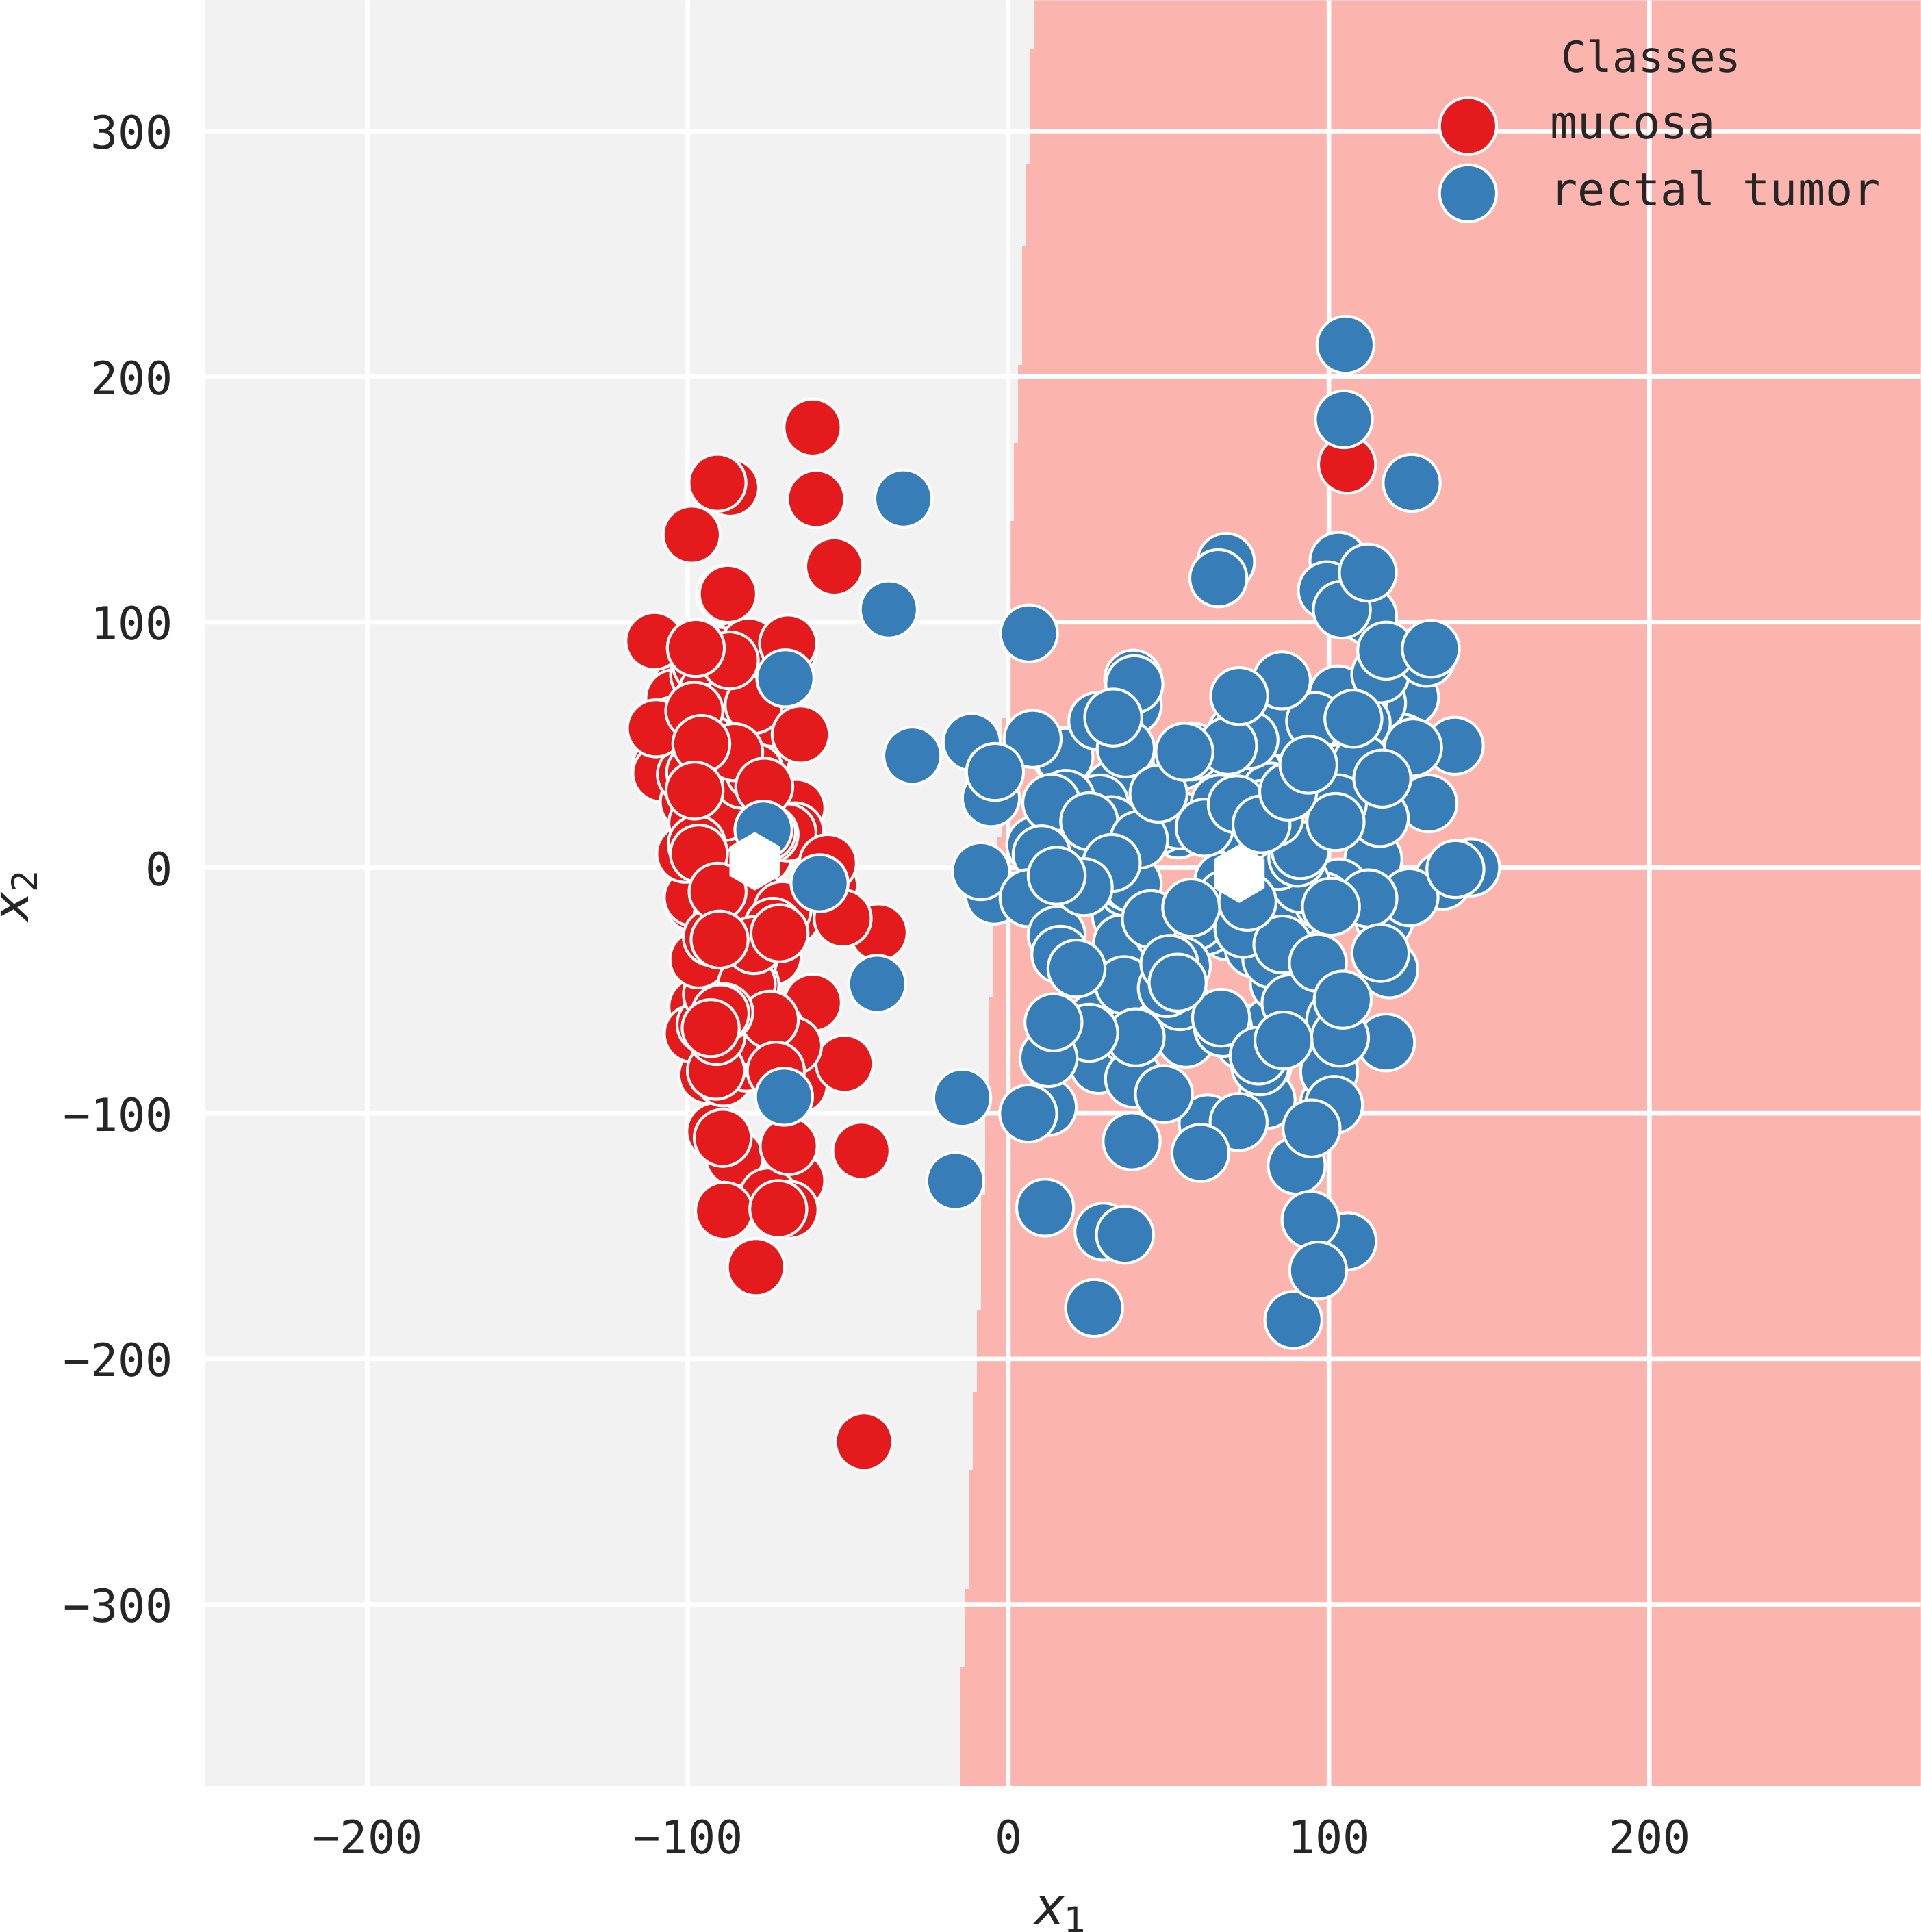
\includegraphics[width=0.32\textwidth]{part2/KMeans_2-clusts_linear.png}
        \label{fig:a}%
    }%
    \hfill%
    \subfloat[]{%
        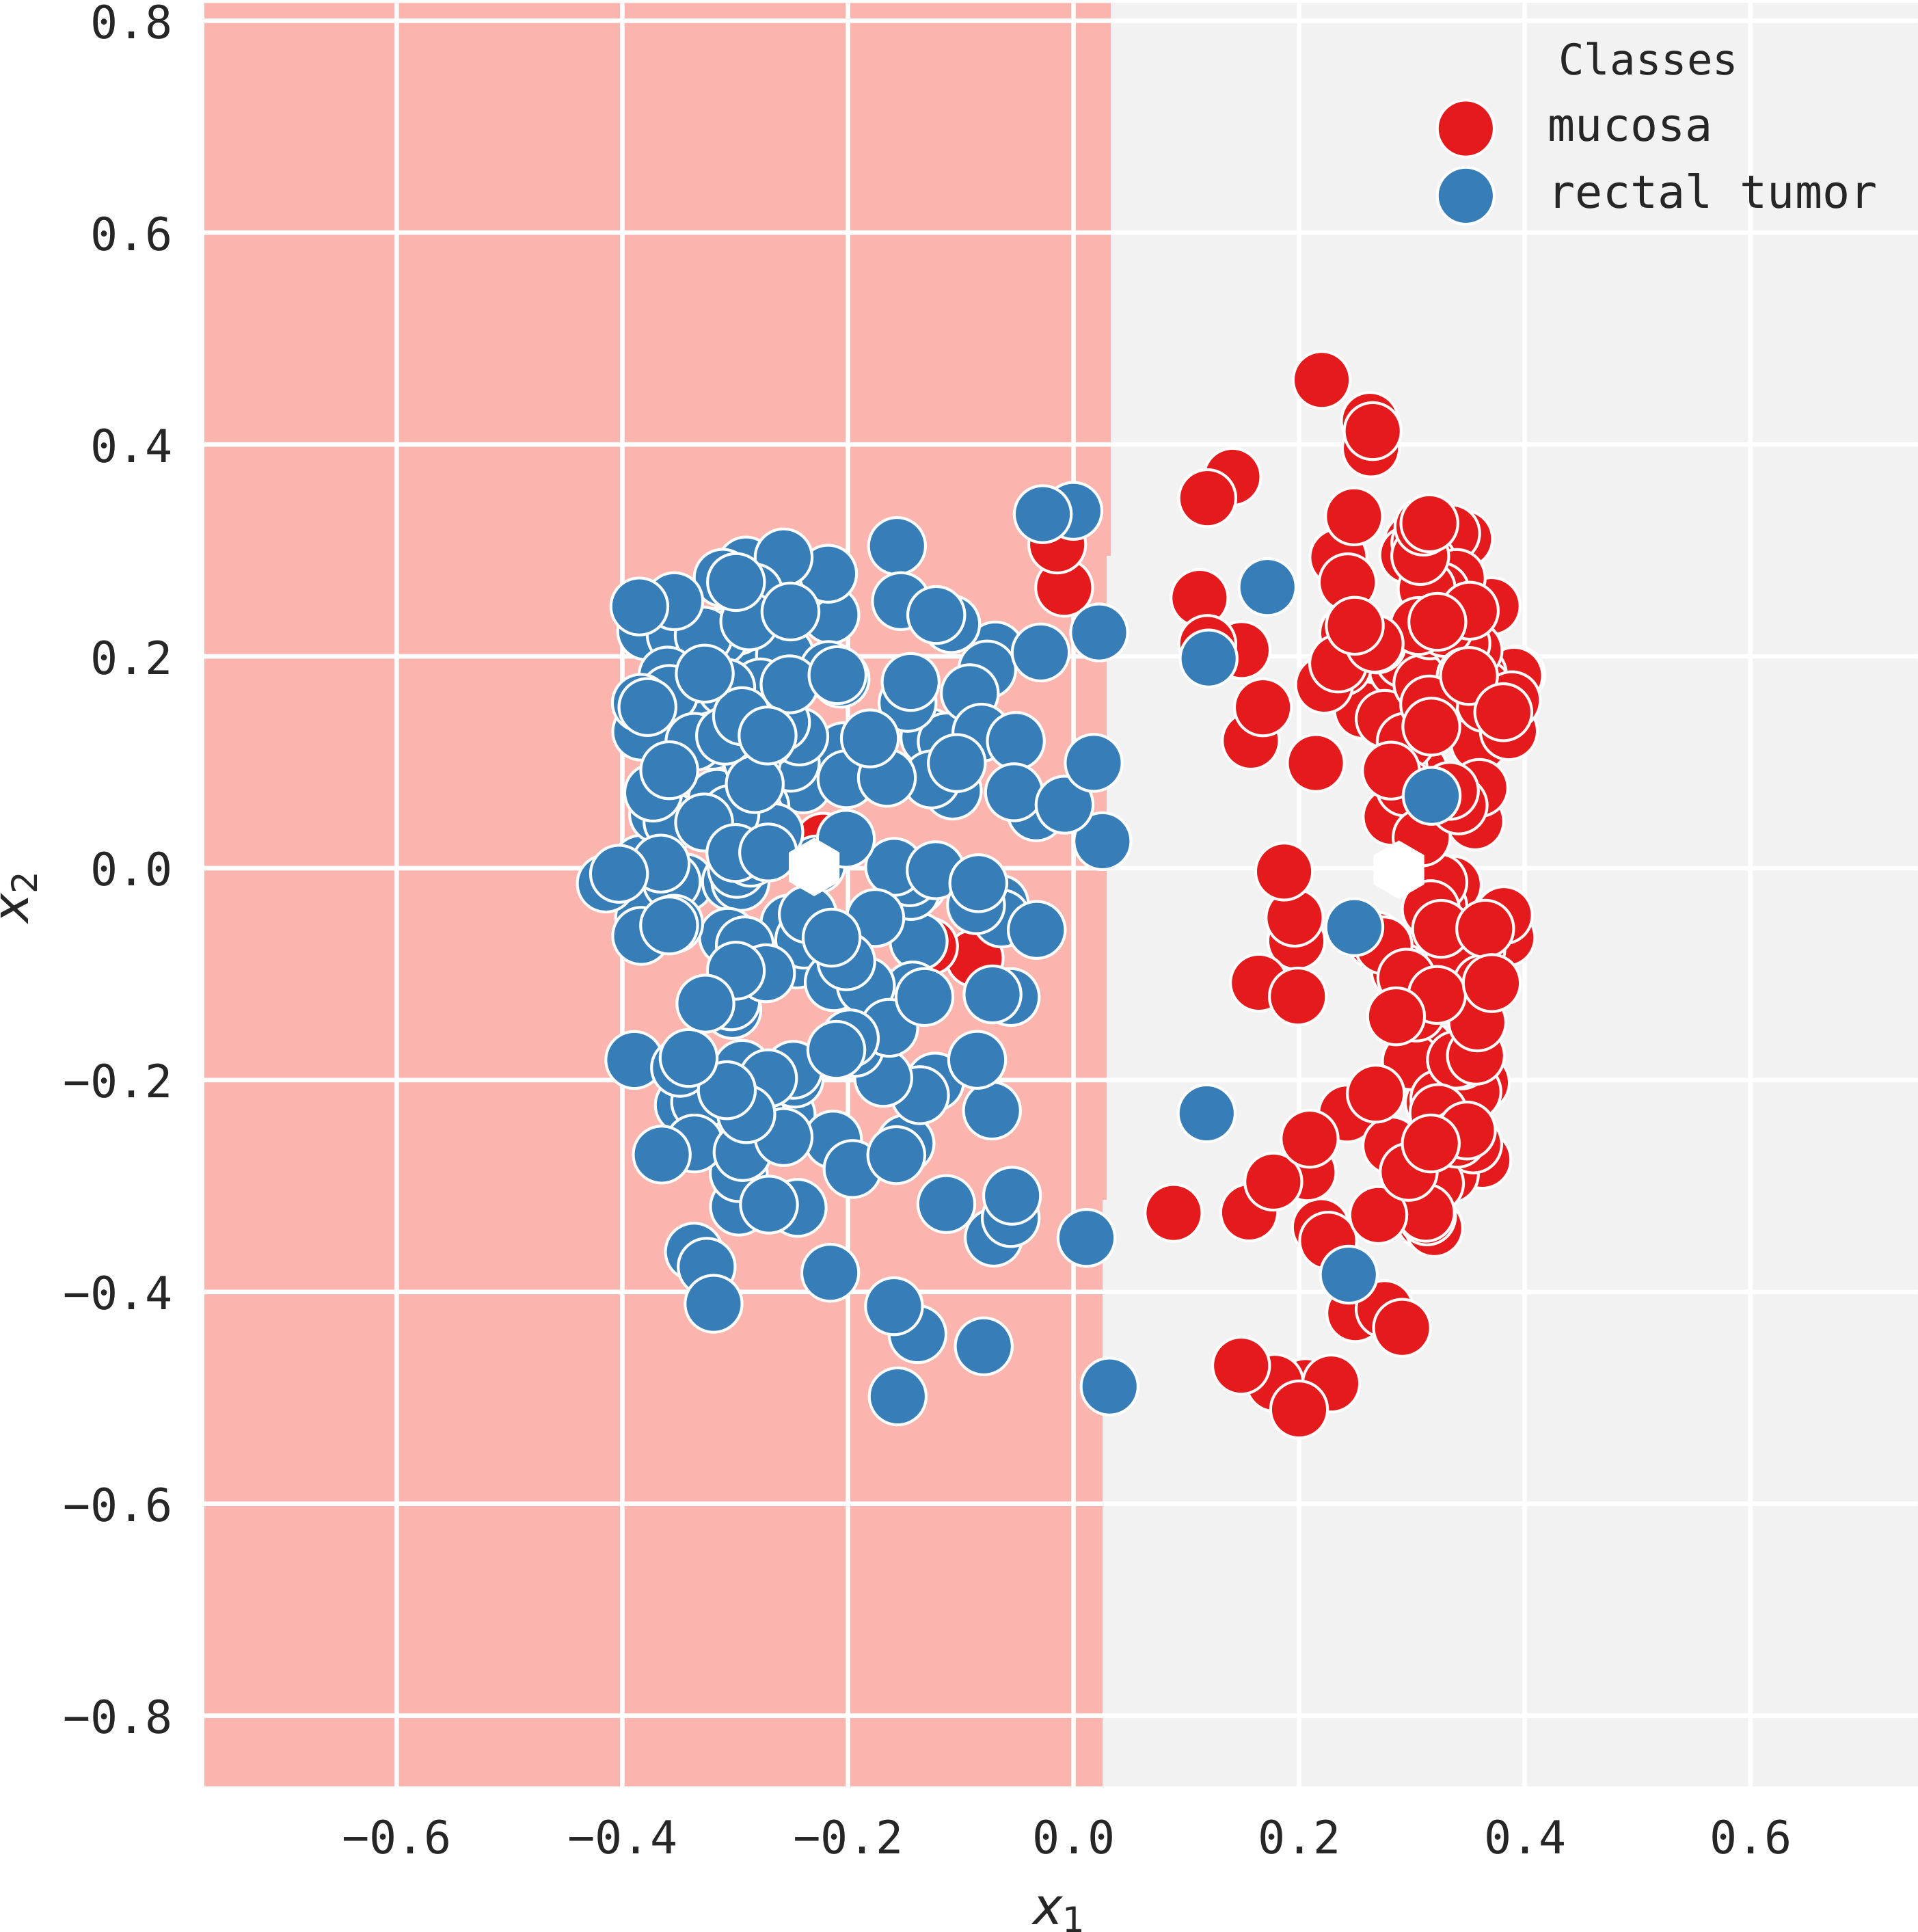
\includegraphics[width=0.32\textwidth]{part2/KMeans_2-clusts_rbf.png}
        \label{fig:b}%
    }%
    \hfill%
    \subfloat[]{%
        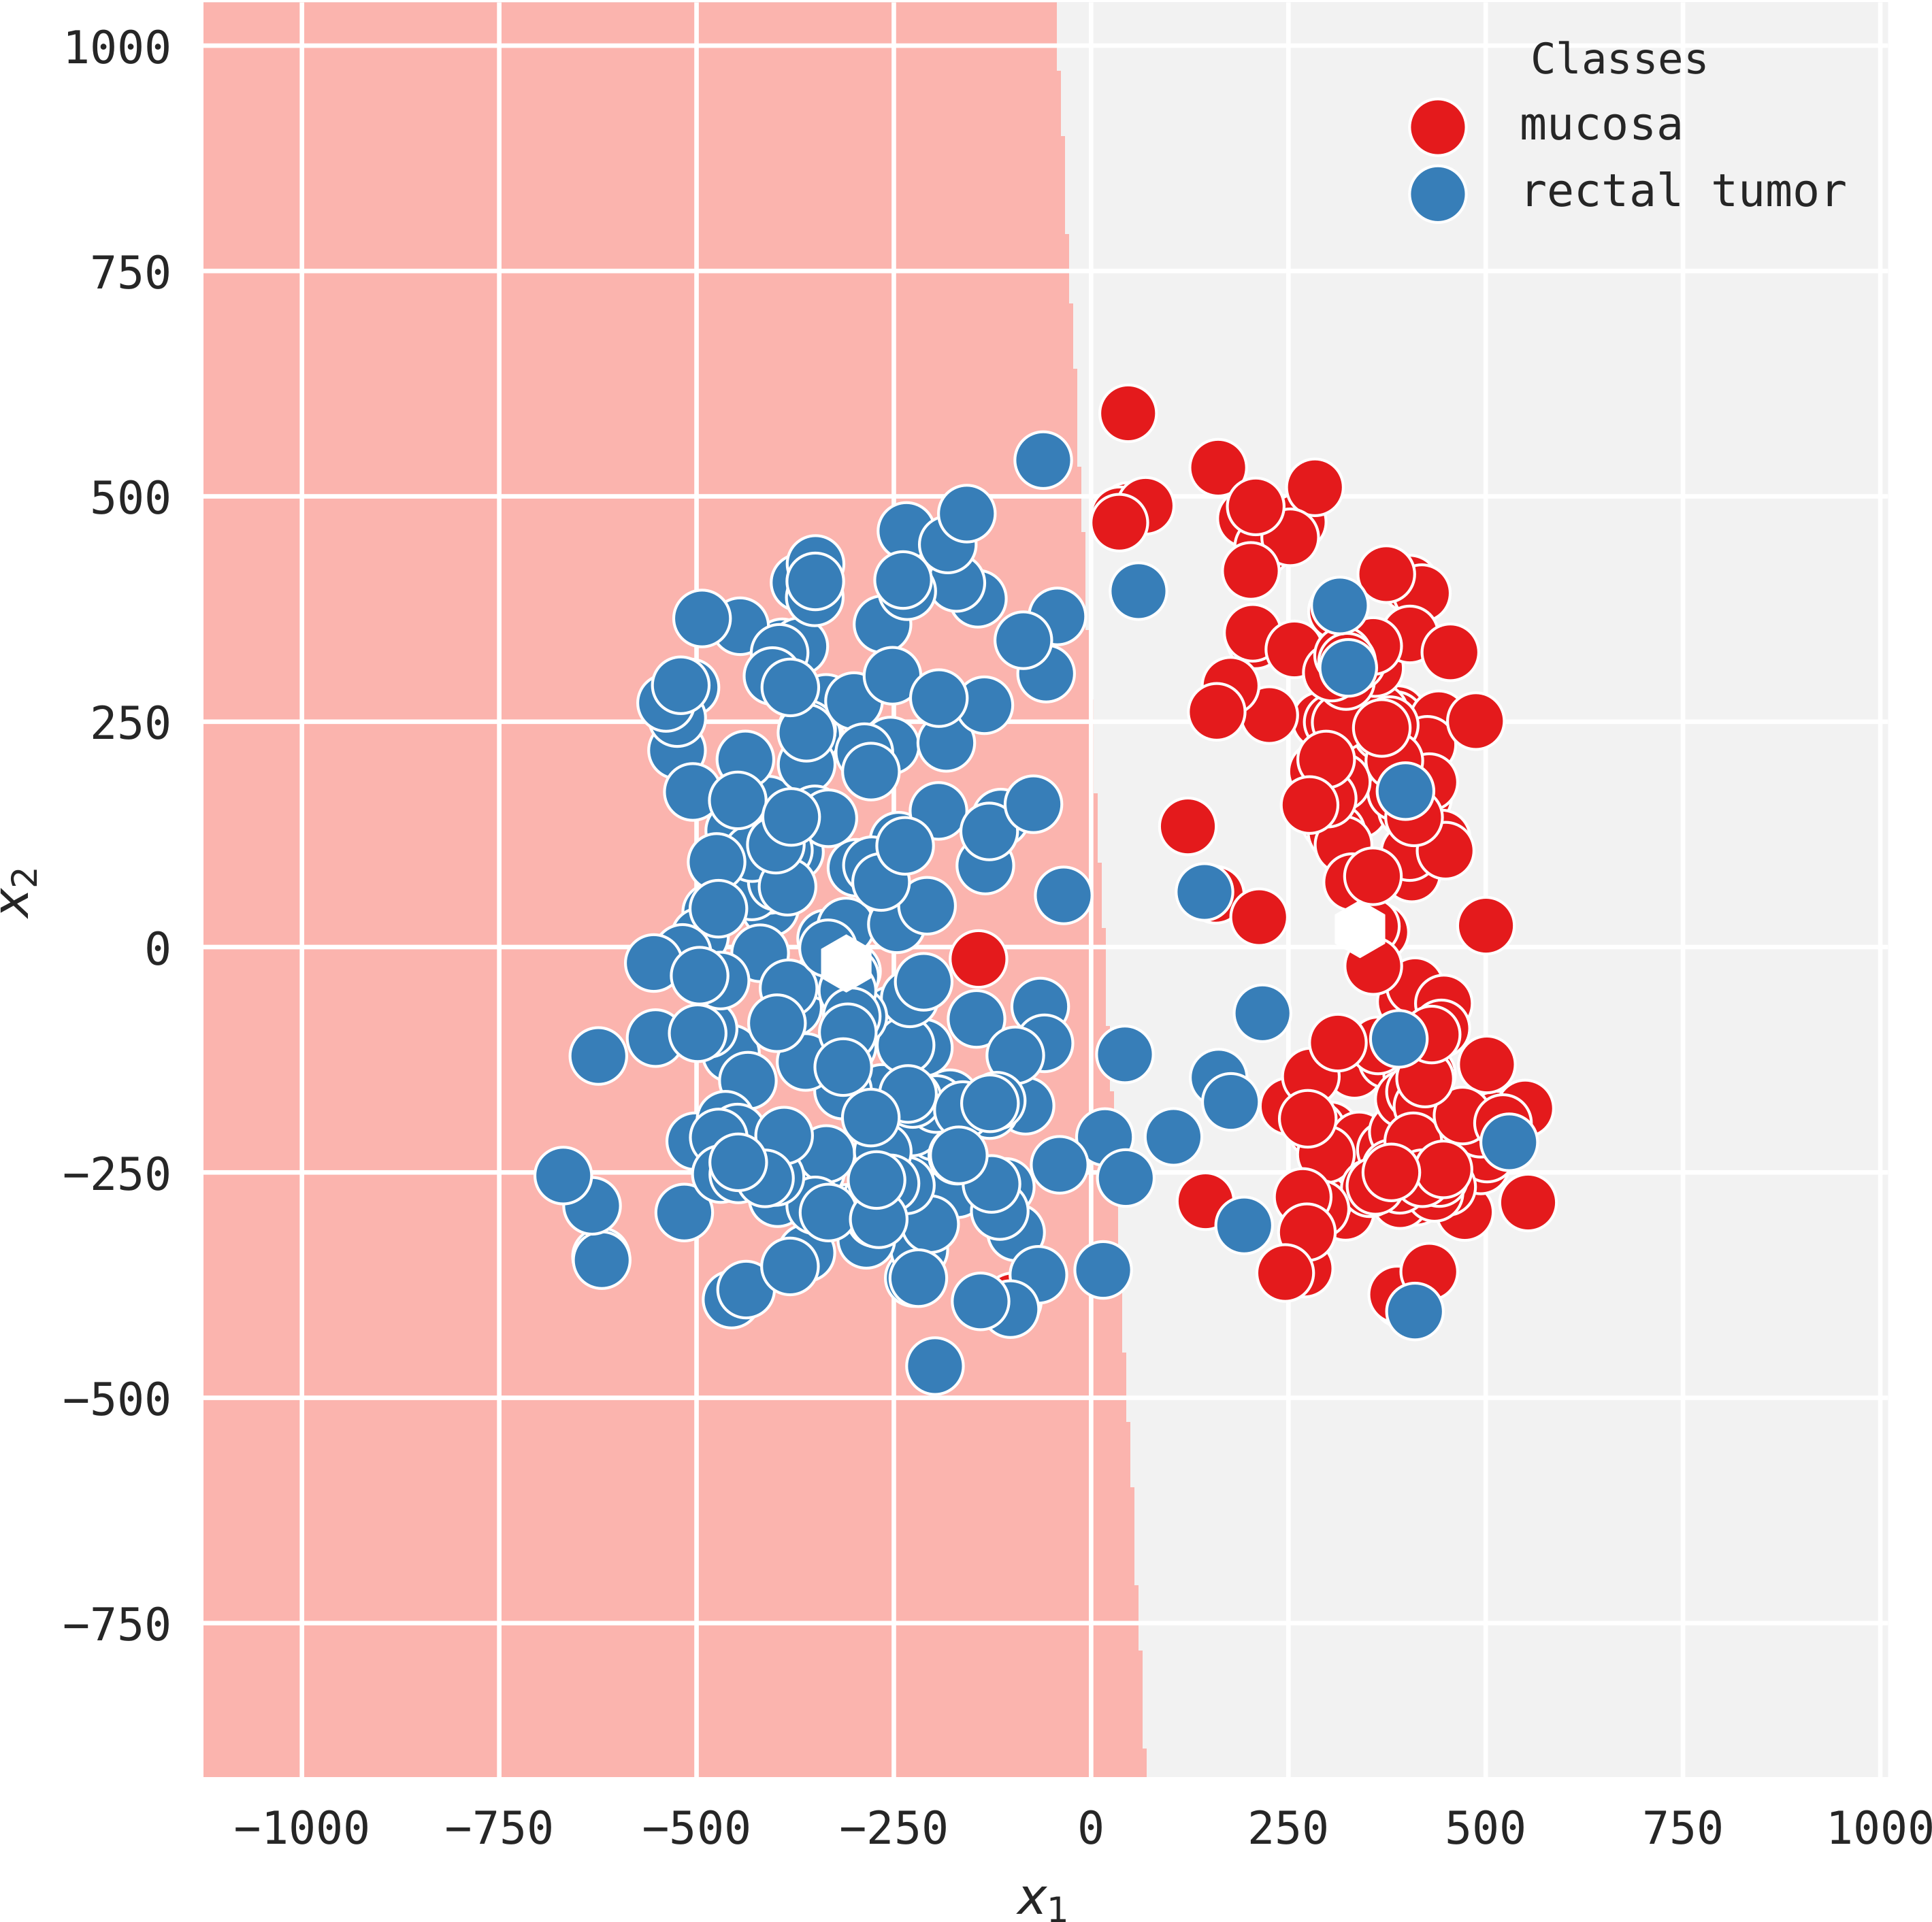
\includegraphics[width=0.32\textwidth]{part2/KMeans_2-clusts_isomap.png}
        \label{fig:c}%
    }%
    \caption{Three different 2D projections of the samples of the GEO gene expression data set used in this work. Projections on the left (a), middle (b) and right (c) panes are obtained via linear PCA, Gaussian PCA and isomap, respectively. The color of each point corresponds to the actual tissue type, while the background color is automatically learned by the $k$-means clustering algorithm. White hexagons correspond to cluster centroids.}\label{fig:scatter}
\end{figure}

For the second EDA, the relationships among the probe sets corresponding to the genes of the signature are separately explored learning a different hierarchical clustering~\cite{hastie2009elements} tree for mucosa (Figures~\ref{fig:mucosatree}) and CRC samples (Figure~\ref{fig:tumortree}), separately.
% shows some differences but some similarities too. This is easy explained by the fact that the mucosa samples derive from the same subjects from which the CRC samples are taken.
% The most evident similarities between these graphs are the following:
% such genes are also closely connected to TP53 and its isoform.
% and GSK3B-MSH2.1
The two trees are learned from different tissues, nevertheless they show some remarkable similarities. For instance, the pairs \tp-\tp{\small .1} and \msh-\pms{\small .1} always share a common parent. Interestingly, the first is a relationship between probe sets of the same gene, and the second is confirmed in literature, as \msh and \pms are both involved in hereditary non-polyposis CRC, a syndrome that predisposes for CRC.
Moreover, two probe sets of the the genes of \emph{S1}, namely \apc and \ctnnb, are consistently close to the root of the two trees. This suggest that the expression level of these two genes highly differs from the others.
% An interesting difference is the position of APC and CTNNB1 with respect to TP53 and its isoform. While in the CRC tree (Figure~\ref{fig:tumortree}) they
% it is evident that there is a direction in the connections of these genes (\ie the first gene is APC, the second is CTNNB1 and the last is TP53 with its isoform) this is not the case for the mucosa tree.
% The position of KRAS with respect to APC and CTNNB1 is another difference that emerges from the comparison of the two graphs: while in the CRC case, KRAS and KRAS.1 are located more or less on the same level in the middle of the graph, the reciprocal position of these two genes is quite different in the mucosa graph. KRAS is positioned close to the bottom of the graph while KRAS.1 is above KRAS and looks quite distant from it.
Two interesting differences between the two trees can also be noticed. First, most of the elements of the sublist \emph{S3}, which contains genes that enhance the risk of developing CRC, tend to be grouped together in Figure~\ref{fig:tumortree}, while the same observation cannot be done for Figure~\ref{fig:mucosatree}. Secondly, probe sets of the genes belonging to sublists \emph{S2} and \emph{S3} tend more to more closely connected in Figure~\ref{fig:tumortree} than in Figure~\ref{fig:mucosatree}.

% The Pearson correlations calculated among all the couples of the considered gene signature, produced two heatmaps one for each tissue type (see Figures XX and XX). From the comparison of these plots it is evident that there is a higher correlation in mucosa with respect to cancer tissue. We expected a clear difference in the appearance of the two heatmaps and the higher correlation in the mucosa samples could be related with the fact that the majority of these samples, disease-free, comes from the same subjects from which the cancer samples are retrieved. Therefore several genes of the signatures looks arelady altered in the mucosa while the same alteration in the tumor is not visible any more because the occurrence of many chromosomal aberrations (e.g., chromosomal translocation, inversions, deletion, gene mutations) it is expected to take place.

\begin{figure}[h!]
    \centering
    \subfloat[]{%
        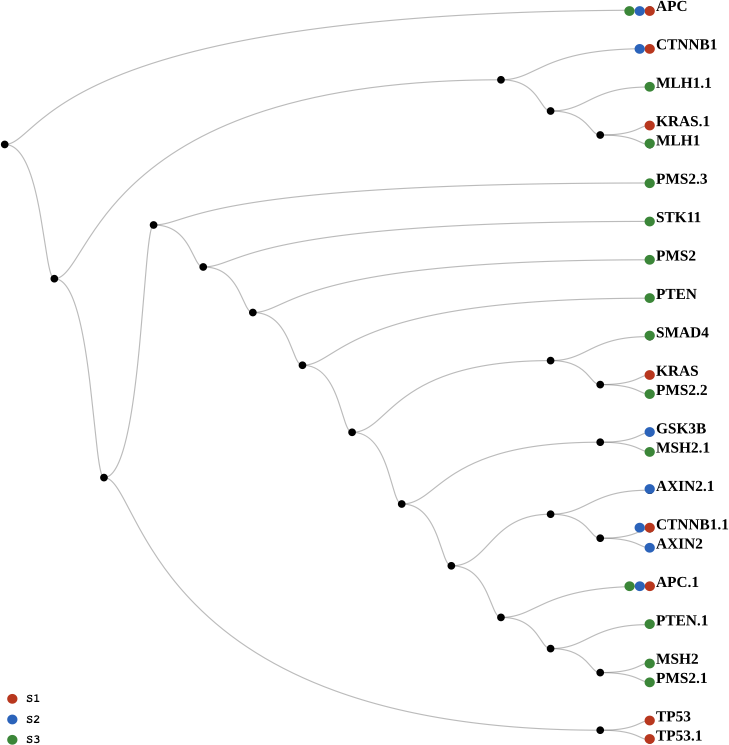
\includegraphics[width=0.45\textwidth]{part2/mucosa_tree_color.png}%
        \label{fig:mucosatree}%
    }%
    \hfill%
    \subfloat[]{%
        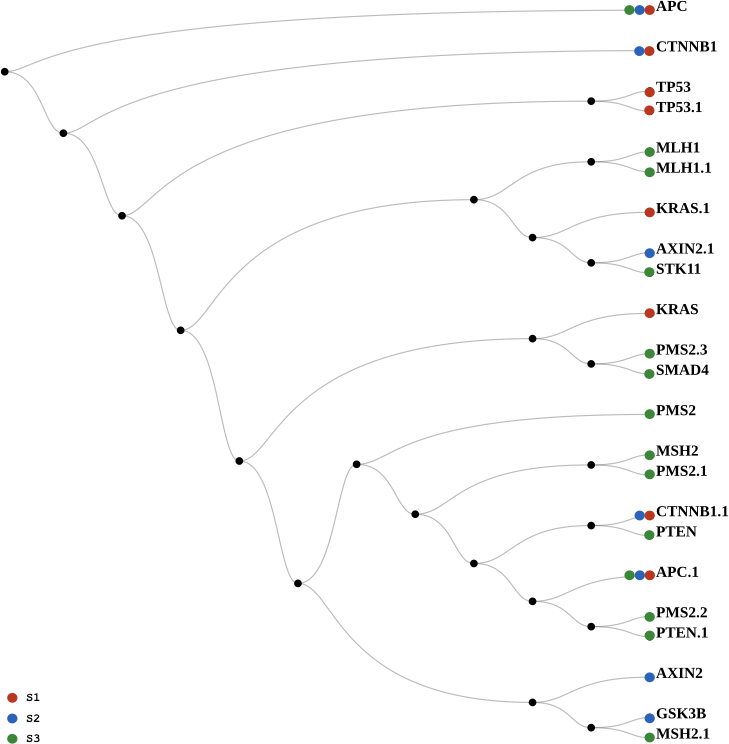
\includegraphics[width=0.45\textwidth]{part2/tumor_tree_color.png}%
        \label{fig:tumortree}%
    }%
    \caption{An example of hierarchical trees visualization learned by two \ade pipelines on mucosa (a) and CRC (b) samples. Each probe set is color coded according to the corresponding sublist. This visualization provides insights on the underlying structure of the measured gene expression level.}\label{fig:trees}
\end{figure}

% Please add the following required packages to your document preamble:
% \usepackage{booktabs}
% \begin{table}[]
%   \footnotesize
% \centering
% \caption{Perfomance summary of the three top performing \ade pipelines. The three pipelines only differ in the dimensionality reduction strategy. {\sl Pipe-1}, {\sl Pipe-2} and {\sl Pipe-3} resort to PCA, Isomap and Gaussian Kernel PCA, respectively}
% \label{tab:performance}
% \begin{tabular}{@{}lrrrr@{}}
% \toprule
% {\bf Pipeline}         & {\bf AMI}             & {\bf Completeness}    & {\bf Homogeneity}     & {\bf Silhouette} \\ \midrule
% \multicolumn{1}{l|}{\sl Pipe-1} & \multicolumn{1}{r|}{0.602} & \multicolumn{1}{r|}{0.603} & \multicolumn{1}{r|}{0.609} & 0.484                 \\
% \multicolumn{1}{l|}{\sl Pipe-2} & \multicolumn{1}{r|}{0.602} & \multicolumn{1}{r|}{0.603} & \multicolumn{1}{r|}{0.608} & 0.555                 \\
% \multicolumn{1}{l|}{\sl Pipe-3} & \multicolumn{1}{r|}{0.565} & \multicolumn{1}{r|}{0.566} & \multicolumn{1}{r|}{0.566} & 0.518 \\
% \bottomrule
% \end{tabular}
% \end{table}

% Pipe1
% median Impute-NaN $\to$ Recenter $\to$ linear KernelPCA $\to$ 2-clusts KMeans
% Pipe2
% median Impute-NaN $\to$ Recenter $\to$ Isomap $\to$ 2-clusts KMeans
% Pip3
% median Impute-NaN $\to$ Recenter $\to$ rbf KernelPCA $\to$ 2-clusts KMeans

%
%In this Chapter we presented \ade, a biomedical data exploration and visualization tool that can seamlessly run on single workstations as well as on HPC clusters.
%Thanks to its scalable architecture, \ade is suitable for the analysis of large and high-dimensional data collections, that are nowadays ubiquitous in biomedicine.
%
%\ade natively supports the integration with the GEO repository. Therefore, a user provided with the accession number of the data set of interest can select target phenotypes and genotypes and \ade takes care of automatically downloading the data and plugging them into the computational framework.
%\ade offers a wide range of missing values imputing, data preprocessing, dimensionality reduction and clustering techniques that can be easily selected and applied to any input data.
%
%In this paper we showed \ade capabilities performing two EDAs on a CRC gene expression data set. From the obtained results we can observe that a clear discrimination between CRC and control samples can be achieved by unsupervised data analysis pipeline.
%% \apc and \ctnnb,
%Moreover, a meaningful description of the relationships among the group of genes strongly associated with CRC can be represented as hierarchical trees.
